\documentclass{vkr}
\usepackage[english, russian]{babel} % переносы
\usepackage{graphicx} % для вставки картинок
\graphicspath{{images/}} % путь к изображениям
\usepackage[hidelinks]{hyperref}
\usepackage{float} % определяет метод H для рисунка с переносом на следующую страницу, ели не помещается
\usepackage{pdflscape}
\addto{\captionsrussian}{\renewcommand{\refname}{СПИСОК ИСПОЛЬЗОВАННЫХ ИСТОЧНИКОВ}}
\usepackage{xltabular} % для вставки таблиц
\usepackage{makecell}
\renewcommand\theadfont{} % шрифт в /thead
\usepackage{array} % для определения новых типов столбцов таблиц
\newcolumntype{T}{>{\centering\arraybackslash}X} % новый тип столбца T - автоматическая ширина столбца с выравниванием по центру
\newcolumntype{R}{>{\raggedleft\arraybackslash}X} % новый тип столбца R - автоматическая ширина столбца с выравниванием по правому краю
\newcolumntype{C}[1]{>{\centering\let\newline\\\arraybackslash\hspace{0pt}}m{#1}} % новый тип столбца C - фиксированная ширина столбца с выравниванием по центру
\newcolumntype{r}[1]{>{\raggedleft\arraybackslash}p{#1}} % новый тип столбца r - фиксированная ширина столбца с выравниванием по правому краю
\newcommand{\centrow}{\centering\arraybackslash} % командой \centrow можно центрировать одну ячейку (заголовок) в столбце типа X или p, оставив в оcтальных ячейках другой тип выравнивания
\newcommand{\finishhead}{\endhead\hline\endlastfoot}
\newcommand{\continuecaption}[1]{\caption*{#1}\\ \hline }
\usepackage{etoolbox}
\AtBeginEnvironment{xltabular}{\refstepcounter{tablecnt}} % подсчет таблиц xltabular, обычные таблицы подсчитываются в классе

\usepackage[tableposition=top]{caption} % подпись таблицы вверху
\captionsetup{strut=off}
\setlength{\intextsep}{0pt} % Vertical space above & below [h] floats
\setlength{\textfloatsep}{0pt} % Vertical space below (above) [t] ([b]) floats
\DeclareCaptionLabelFormat{gostfigure}{Рисунок #2} %подпись рисунка
\DeclareCaptionLabelFormat{gosttable}{Таблица #2} %подпись таблицы
\DeclareCaptionLabelSeparator{gost}{~--~} %разделитель в рисунках и таблицах
\captionsetup{labelsep=gost}
\captionsetup[figure]{aboveskip=10pt,belowskip=4mm,justification=centering,labelformat=gostfigure} % настройка подписи рисунка
\captionsetup[table]{font={stretch=1.41},skip=0pt,belowskip=0pt,aboveskip=8.5pt,singlelinecheck=off,labelformat=gosttable} % настройка подписи таблицы

\setlength{\LTpre}{8mm} % отступ сверху таблицы
\setlength{\LTpost}{6mm} % отступ снизу таблицы

\usepackage{enumitem}
\setlist{nolistsep,wide=\parindent,itemindent=*} % отступы вокруг списков, выравнивание с учетом разделителя

\usepackage{color} %% это для отображения цвета в коде
\usepackage{listings} %% листинги кода
\setmonofont[Scale=0.7]{Verdana} % моноширный шрифт для листинга

\definecolor{codegreen}{rgb}{0,0.6,0}
\definecolor{codegray}{rgb}{0.5,0.5,0.5}
\definecolor{codepurple}{rgb}{0.58,0,0.82}

\lstset{ %
language=C,                 % выбор языка для подсветки (здесь это С)
numbers=left,               % где поставить нумерацию строк (слева\справа)
numberstyle=\tiny,           % размер шрифта для номеров строк
stepnumber=1,                   % размер шага между двумя номерами строк
numbersep=5pt,                % как далеко отстоят номера строк от подсвечиваемого кода
commentstyle=\color{codegreen},
keywordstyle=\color{magenta},
numberstyle=\tiny\color{codegray},
stringstyle=\color{codepurple},
basicstyle=\linespread{0.95}\ttfamily,
backgroundcolor=\color{white}, % цвет фона подсветки - используем \usepackage{color}
showspaces=false,            % показывать или нет пробелы специальными отступами
showstringspaces=false,      % показывать или нет пробелы в строках
showtabs=false,             % показывать или нет табуляцию в строках
frame=single,              % рисовать рамку вокруг кода
tabsize=2,                 % размер табуляции по умолчанию равен 2 пробелам
captionpos=t,              % позиция заголовка вверху [t] или внизу [b] 
breaklines=true,           % автоматически переносить строки (да\нет)
breakatwhitespace=false, % переносить строки только если есть пробел
escapeinside={\%*}{*)}   % если нужно добавить комментарии в коде
}

\makeatletter % чтобы допускались русские комментарии в листингах
\lst@InputCatcodes
\def\lst@DefEC{%
 \lst@CCECUse \lst@ProcessLetter
  ^^80^^81^^82^^83^^84^^85^^86^^87^^88^^89^^8a^^8b^^8c^^8d^^8e^^8f%
  ^^90^^91^^92^^93^^94^^95^^96^^97^^98^^99^^9a^^9b^^9c^^9d^^9e^^9f%
  ^^a0^^a1^^a2^^a3^^a4^^a5^^a6^^a7^^a8^^a9^^aa^^ab^^ac^^ad^^ae^^af%
  ^^b0^^b1^^b2^^b3^^b4^^b5^^b6^^b7^^b8^^b9^^ba^^bb^^bc^^bd^^be^^bf%
  ^^c0^^c1^^c2^^c3^^c4^^c5^^c6^^c7^^c8^^c9^^ca^^cb^^cc^^cd^^ce^^cf%
  ^^d0^^d1^^d2^^d3^^d4^^d5^^d6^^d7^^d8^^d9^^da^^db^^dc^^dd^^de^^df%
  ^^e0^^e1^^e2^^e3^^e4^^e5^^e6^^e7^^e8^^e9^^ea^^eb^^ec^^ed^^ee^^ef%
  ^^f0^^f1^^f2^^f3^^f4^^f5^^f6^^f7^^f8^^f9^^fa^^fb^^fc^^fd^^fe^^ff%
  ^^^^20ac^^^^0153^^^^0152%
  % Basic Cyrillic alphabet coverage
  ^^^^0410^^^^0411^^^^0412^^^^0413^^^^0414^^^^0415^^^^0416^^^^0417%
  ^^^^0418^^^^0419^^^^041a^^^^041b^^^^041c^^^^041d^^^^041e^^^^041f%
  ^^^^0420^^^^0421^^^^0422^^^^0423^^^^0424^^^^0425^^^^0426^^^^0427%
  ^^^^0428^^^^0429^^^^042a^^^^042b^^^^042c^^^^042d^^^^042e^^^^042f%
  ^^^^0430^^^^0431^^^^0432^^^^0433^^^^0434^^^^0435^^^^0436^^^^0437%
  ^^^^0438^^^^0439^^^^043a^^^^043b^^^^043c^^^^043d^^^^043e^^^^043f%
  ^^^^0440^^^^0441^^^^0442^^^^0443^^^^0444^^^^0445^^^^0446^^^^0447%
  ^^^^0448^^^^0449^^^^044a^^^^044b^^^^044c^^^^044d^^^^044e^^^^044f%
  ^^^^0401^^^^0451%
  %%%
  ^^00}
\lst@RestoreCatcodes
\makeatother


% Режим шаблона (должен быть включен один из трех)
%\ВКРtrue
\Практикаtrue
%\Курсоваяtrue

\newcommand{\Дисциплина}{-} % для курсовой
\newcommand{\КодСпециальности}{09.03.04} % Курсовая
\newcommand{\Специальность}{Программная инженерия} % Курсовая
\newcommand{\Тема}{Бизнес-проект «Веб-приложение «КиТ» для сбора и анализа информации об инцидентах с общественным транспортом». Микросервис «Работа с обращениями граждан»} % ВКР Курсовая
\newcommand{\ТемаВтораяСтрока}{-}
\newcommand{\ГдеПроводитсяПрактика}{ОБУ «Курскгражданпроект»} % для практики
\newcommand{\РуководительПрактПредпр}{Пахомов Е. И.} % для практики
\newcommand{\ДолжнРуководительПрактПредпр}{зам.директора по производству} % для практики
\newcommand{\РуководительПрактУнивер}{Чаплыгин А. А.} % для практики
\newcommand{\ДолжнРуководительПрактУнивер}{к.т.н. доцент} % для практики
\newcommand{\Автор}{А. В. Гуляева}
\newcommand{\АвторРод}{Гуляевой А.В.}
\newcommand{\АвторПолностьюРод}{Гуляевой Александры Викторовны} % для практики
\newcommand{\Шифр}{20-06-0114}
\newcommand{\Курс}{4 } % для практики
\newcommand{\Группа}{ПО-01б}
\newcommand{\Руководитель}{А. А. Чаплыгин} % для ВКР и курсовой
\newcommand{\Нормоконтроль}{А. А. Чаплыгин} % для ВКР
\newcommand{\ЗавКаф}{А. В. Малышев} % для ВКР
\newcommand{\ДатаПриказа}{«**» апреля 2024~г.} % для ВКР
\newcommand{\НомерПриказа}{****-с} % для ВКР
\newcommand{\СрокПредоставления}{«**» мая 2024~г.} % для ВКР, курсового

\begin{document}
\maketitle
\ifПрактика{}\else{
   \newpage
\begin{center}
\large\textbf{Минобрнауки России}

\large\textbf{Юго-Западный государственный университет}
\vskip 1em
\normalsize{Кафедра программной инженерии}
\vskip 1em
\ifВКР{
        \begin{flushright}
        \begin{tabular}{p{.4\textwidth}}
        \centrow УТВЕРЖДАЮ: \\
        \centrow Заведующий кафедрой \\
        \hrulefill \\
        \setarstrut{\footnotesize}
        \centrow\footnotesize{(подпись, инициалы, фамилия)}\\
        \restorearstrut
        «\underline{\hspace{1cm}}»
        \underline{\hspace{3cm}}
        20\underline{\hspace{1cm}} г.\\
        \end{tabular}
        \end{flushright}
        }\fi
\end{center}
\vspace{1em}
  \begin{center}
  \large
\ifВКР{
ЗАДАНИЕ НА ВЫПУСКНУЮ КВАЛИФИКАЦИОННУЮ РАБОТУ
  ПО ПРОГРАММЕ БАКАЛАВРИАТА}
  \else
ЗАДАНИЕ НА КУРСОВУЮ РАБОТУ (ПРОЕКТ)
\fi
\normalsize
  \end{center}
\vspace{1em}
{\parindent0pt
  Студента \АвторРод, шифр\ \Шифр, группа \Группа
  
1. Тема «\Тема\ \ТемаВтораяСтрока»
\ifВКР{
утверждена приказом ректора ЮЗГУ от \ДатаПриказа\ № \НомерПриказа
}\fi.

2. Срок предоставления работы к защите \СрокПредоставления

3. Исходные данные для создания программной системы:

3.1. Перечень решаемых задач:}

\renewcommand\labelenumi{\theenumi)}

\begin{enumerate}
\item проанализировать IT-инфраструктуру предприятия;
\item  разработать концептуальную модель системы управления IT-ин\-фра\-струк\-турой предприятия на основе подхода к управлению и организации ИТ-услуг ITSM;
\item спроектировать программную систему управления IT-ин\-фра\-струк\-турой предприятия;
\item сконструировать и протестировать программную систему управления IT-инфраструктурой предприятия.
\end{enumerate}

{\parindent0pt
  3.2. Входные данные и требуемые результаты для программы:}

\begin{enumerate}
\item Входными данными для программной системы являются: данные
справочников комплектующих, конфигураций, ПО, критериев качества SLA,
ИТ-услуг, департаментов компании; технические данные ИТ-ресурсов; данные входящих заявок на ИТ-ресурсы; данные запросов поставщикам на комплектующие.
\item Выходными данными для программной системы являются: сформированные заявки на обслуживание ИТ-ресурсов; сформированные запросы на
закупку комплектующих; сведения о выполненных работах по заявкам; статусы заявок; выходные отчеты (инфографика) – по качеству услуг, по состоянию ИТ-ресурсов, по деятельности ИТ-отдела, по стоимости обслуживания
ИТ-ресурсов, воронка заявок.
\end{enumerate}

{\parindent0pt

  4. Содержание работы (по разделам):
  
  4.1. Введение
  
  4.1. Анализ предметной области
  
4.2. Техническое задание: основание для разработки, назначение разработки,
требования к программной системе, требования к оформлению документации.

4.3. Технический проект: общие сведения о программной системе, проект
данных программной системы, проектирование архитектуры программной системы, проектирование пользовательского интерфейса программной системы.

4.4. Рабочий проект: спецификация компонентов и классов программной системы, тестирование программной системы, сборка компонентов программной системы.

4.5. Заключение

4.6. Список использованных источников

5. Перечень графического материала:

\списокПлакатов

\vskip 2em
\begin{tabular}{p{6.8cm}C{3.8cm}C{4.8cm}}
Руководитель \ifВКР{ВКР}\else работы (проекта) \fi & \lhrulefill{\fill} & \fillcenter\Руководитель\\
\setarstrut{\footnotesize}
& \footnotesize{(подпись, дата)} & \footnotesize{(инициалы, фамилия)}\\
\restorearstrut
Задание принял к исполнению & \lhrulefill{\fill} & \fillcenter\Автор\\
\setarstrut{\footnotesize}
& \footnotesize{(подпись, дата)} & \footnotesize{(инициалы, фамилия)}\\
\restorearstrut
\end{tabular}
}

\renewcommand\labelenumi{\theenumi.}

   \abstract{РЕФЕРАТ}

Объем работы равен \formbytotal{lastpage}{страниц}{е}{ам}{ам}. Работа содержит \formbytotal{figurecnt}{иллюстраци}{ю}{и}{й}, \formbytotal{tablecnt}{таблиц}{у}{ы}{}, \arabic{bibcount} библиографических источников и \formbytotal{числоПлакатов}{лист}{}{а}{ов} графического материала. Количество приложений – 2. Графический материал представлен в приложении А. Фрагменты исходного кода представлены в приложении Б.

Перечень ключевых слов: коммерческий сайт, Система, CMS, Битрикс, Joomla, аддитивные технологии, 3D-принтеры, услуги, сервисы, информатизация, автоматизация, информационные технологии, веб-форма,  Apache, классы, база данных, средства защиты информации, подсистема, компонент, модуль, сущность, информационный блок, метод, контент-редактор, администратор, пользователь, web-сайт.

Объектом разработки является web-сайт компании,  занимающейся производством 3D-принтеров, выпуском оборудования для создания порошков, разработкой программного обеспечения и организацией центров аддитивного производства.

Целью выпускной квалификационной работы является привлечение клиентов, увеличение заказов, информирование о продукции и услугах путем создания сайта компании.

В процессе создания сайта были выделены основные сущности путем создания информационных блоков, использованы классы и методы модулей, обеспечивающие работу с сущностями предметной области, а также корректную работу web-сайта, разработаны разделы, содержащие информацию о компании, ее деятельности, производимой продукции и услугах, разработан сервис по заказу 3D-деталей.

При разработке сайта использовалась система управления контентом "<1С-Битрикс: Управление сайтом">.

Разработанный сайт был успешно внедрен в компании.

\selectlanguage{english}
\abstract{ABSTRACT}
  
The volume of work is \formbytotal{lastpage}{page}{}{s}{s}. The work contains \formbytotal{figurecnt}{illustration}{}{s}{s}, \formbytotal{tablecnt}{table}{}{s}{s}, \arabic{bibcount} bibliographic sources and \formbytotal{числоПлакатов}{sheet}{}{s}{s} of graphic material. The number of applications is 2. The graphic material is presented in annex A. The layout of the site, including the connection of components, is presented in annex B.

List of keywords: commercial website, System, CMS, Bitrix, Joomla, additive technologies, 3D printers, services, services, informatization, automation, information technology, web form, Apache, classes, database, component, module, entity, information block, method, content editor, administrator, user, web site.

The object of the research is the analysis of information technologies for the development of a production company's website.

The object of the development is the website of a company engaged in the production of 3D printers, the production of equipment for the creation of powders, software development and the organization of additive manufacturing centers.

The purpose of the final qualifying work is to attract customers, increase orders, inform about products and services by creating a company website.

In the process of creating the site, the main entities were identified by creating information blocks, classes and methods of modules were used to ensure work with the entities of the subject area, as well as the correct operation of the website, sections containing information about the company, its activities, products and services were developed, a service for ordering 3D parts was developed.

When developing the site, the content management system <<1C – Bitrix: Site Management>> was used.

The developed website was successfully implemented in the company.
\selectlanguage{russian}
}\fi
\tableofcontents
%\section*{ОБОЗНАЧЕНИЯ И СОКРАЩЕНИЯ}

БД -- база данных.

ИС -- информационная система.

ИТ -- информационные технологии. 

КТС -- комплекс технических средств.

ОМТС -- отдел материально-технического снабжения. 

ПО -- программное обеспечение.

РП -- рабочий проект.

СУБД -- система управления базами данных.

ТЗ -- техническое задание.

ТП -- технический проект.

UML (Unified Modelling Language) -- язык графического описания для объектного моделирования в области разработки программного обеспечения.

\ifПрактика{}\else{\section*{ВВЕДЕНИЕ}
\addcontentsline{toc}{section}{ВВЕДЕНИЕ}

Аддитивные технологии (АТ) начали активно развиваться со времени получения первых трехмерных изображений изделий на дисплеях компьютеров. Начало положила стереолитография, затем довольно многочисленные новые принципы стали называть технологиями быстрого прототипирования, затем укоренилось название "<Аддитивные технологии">. Интенсивность развития данных технологий не имеет аналогов. АТ изменили процессы проектирования и конструирования изделий, превратив их в процессы непрерывного создания изделий. Современные проектирование и производство изделий невозможно представить без данного рода технологий. 3D-принтеры стали такими же распространенными, как и персональные компьютеры. С помощью 3D-принтеров получают ткани, обувь, продукты питания, а также выращивают человеческие органы. Во многих отраслях, например, в космической отрасли, альтернативы аддитивным технологиям нет.

АТ предполагают изготовление детали методом послойного нанесения материала, в отличие от традиционных методов формирования детали, за счёт удаления материала из массива заготовки.

При использовании АТ все стадии реализации проекта от идеи до материализации находятся в единой технологической цепи, в которой каждая технологическая операция выполняется в цифровой CAD/CAM/CAE-системе.

Современные компании, видя, как развиваются информационные технологии, пытаются использовать их выгодно для своего бизнеса, поэтому запускают свой web-сайт. С его помощью предприятие может заявить о себе, проинформировать потенциального заказчика об услугах или продуктах, которые предоставляет, а также позволяет пользователям сделать с помощью сайта онлайн-заказ, произвести покупку или оплатить счета.

Сайт считается лицом компании и может существенно повысить ее имидж. Любой пользователь сети Интернет сможет получить необходимую информацию о компании в любой момент, появляется возможность найти контактные телефоны, адрес и e-mail, чтобы связаться с компанией. Сейчас большинство клиентов узнают о ее существовании именно через сайт. Поэтому сайт можно назвать самой лучшей рекламой. 

Главной задачей профессионально построенного сайта является превращение посетителя, зашедшего на сайт, в потенциального клиента.

\emph{Цель настоящей работы} – разработка web-сайта компании для привлечения новой аудитории, увеличения заказов, рекламы продукции и услуг компании. Для достижения поставленной цели необходимо решить \emph{следующие задачи:}
\begin{itemize}
\item провести анализ предметной области;
\item разработать концептуальную модель web-сайта;
\item спроектировать web-сайт;
\item реализовать сайт средствами web-технологий.
\end{itemize}

\emph{Структура и объем работы.} Отчет состоит из введения, 4 разделов основной части, заключения, списка использованных источников, 2 приложений. Текст выпускной квалификационной работы равен \formbytotal{page}{страниц}{е}{ам}{ам}.

\emph{Во введении} сформулирована цель работы, поставлены задачи разработки, описана структура работы, приведено краткое содержание каждого из разделов.

\emph{В первом разделе} на стадии описания технической характеристики предметной области приводится сбор информации о деятельности компании, для которой осуществляется разработка сайта.

\emph{Во втором разделе} на стадии технического задания приводятся требования к разрабатываемому сайту.

\emph{В третьем разделе} на стадии технического проектирования представлены проектные решения для web-сайта.

\emph{В четвертом разделе} приводится список классов и их методов, использованных при разработке сайта, производится тестирование разработанного сайта.

В заключении излагаются основные результаты работы, полученные в ходе разработки.

В приложении А представлен графический материал.
В приложении Б представлены фрагменты исходного кода. 
}\fi
\section{Анализ предметной области}
\subsection{Общественный транспорт и его роль в жизни города}

Перевозка людей на транспорте является ответственной и важной работой в жизни города. Ежедневно сотни тысяч людей используют общественный транспорт, чтобы добраться из пункта А в пункт Б. Благодаря городскому транспорту люди без труда могут доехать до места работы, учебы, медицинских учреждений или совершить поездку по своим делам. К общественному транспорту относятся:
\begin{itemize}
	\item Автобусы -- один из самых распространенных видов городского общественного транспорта. Автобусы следуют по определенным маршрутам и останавливаются на остановках для посадки и высадки пассажиров.
	\item Трамваи -- электрические транспортные средства, движущиеся по рельсам. Трамваи также следуют по установленным маршрутам.
	\item Метро -- подземный или надземный железнодорожный транспорт, обычно имеющий несколько линий и станций. Метро обеспечивает быстрое и эффективное передвижение в городе, особенно в крупных мегаполисах.
	\item Поезда -- большинство городов имеют железнодорожное сообщение, которое обеспечивает связь между ними.
	\item Троллейбусы -- электрические транспортные средства, которые движутся по улицам города, питаясь электричеством от воздушной контактной сети, установленной над дорогами. Троллейбусы также следуют по установленным маршрутам.
	\item Маршрутные такси (маршрутки) -- небольшие пассажирские автобусы или микроавтобусы, следующие по установленным маршрутам, но обычно имеющие более гибкий график и маршрут, чем обычные автобусы.
	\item Такси -- услуга пассажирского транспорта, предоставляемая частными лицами или специализированными компаниями. Такси обычно предоставляет индивидуальные или групповые поездки на короткие и средние расстояния в пределах города или за его пределами.
\end{itemize}

 Разновидностей городского транспорта много, каждый имеет свои преимущества и недостатки. Любой человек может выбрать тот вид транспорта, который ему наиболее удобен. Общественный транспорт играет важную роль в жизни города, поэтому услуги перевозки людей на транспорте должны выполняться качественно и безопасно как для самих пассажиров, так и для других участников дорожного движения города.

\subsection{Преимущества и недостатки общественного транспорта -- Автобусы}

Автобусы являются основным видом общественного транспорта в жизни города. Они имеют следующие преимущества:
\begin{itemize}
	\item Общедоступность. Автобусы предоставляют широкий охват маршрутов, что делает их доступными для большого количества жителей города. Это особенно важно для обслуживания пригородных и отдаленных районов, где другие формы общественного транспорта могут быть менее эффективны.
	\item Экономическая эффективность. Автобусы, как правило, имеют более низкие затраты на инфраструктуру по сравнению с другими формами общественного транспорта, такими как метро или трамвайные системы.
	\item Гибкость. Автобусы легче адаптировать к изменениям в маршрутах и времени движения, что делает их гибкими в управлении и обеспечении обслуживания в тех местах, где они наиболее необходимы.
	\item Интермодальность. Автобусы интегрируются в систему общественного транспорта, что позволяет пассажирам пересаживаться с одного вида транспорта на другой для удобства перемещения по городу.
	\item Экологическая устойчивость. Некоторые автобусы работают на альтернативных источниках энергии, таких как электричество или биотопливо, что делает их более экологически чистыми по сравнению с автомобилями, работающими на бензине или дизеле.
	\item Социальная интеграция. Автобусы способствуют социальной интеграции, предоставляя возможность перемещения для всех слоев населения, включая тех, кто не может себе позволить собственный автомобиль или другие виды транспорта.
\end{itemize}

У автобусов помимо преимуществ, также есть и недостатки:
\begin{itemize}
	\item Задержки. Иногда автобусы застревают в пробках, особенно в перегруженных городских центрах, что приводит к сбоям в графике движения и недовольству пассажиров.
	\item Негативное воздействие на окружающую среду и шум. Движение автобусов может вызывать загрязнение воздуха и шум, особенно при использовании дизельных двигателей, что наносит непоправимый вред экологии и здоровью пассажиров.
	\item Ограниченная вместимость. Автобусы имеют ограниченное количество сидячих мест, поэтому в периоды пиковой нагрузки они могут быть переполнены, что вызывает дискомфорт и неудобства для пассажиров.
	\item Безопасность. В сравнении с другими видами транспорта, такими как метро или поезда, автобусы могут представлять больший риск для безопасности, особенно при авариях на дорогах или в случае неправильного поведения пассажиров или других участников дорожного движения.
	\item Ограниченная скорость. Автобусы обычно движутся медленнее, чем другие виды транспорта, особенно в городах с высоким трафиком, что может сделать их менее привлекательными для тех, кто ценит скорость, удобство и время.
	\item Ограниченность маршрутов. В некоторых городах автобусные маршруты могут быть ограничены, в следствии чего, некоторые районы могут оставаться недоступными или иметь ограниченное обслуживание, особенно в ночное время или по выходным дням.
	\item Комфорт и удобство. В сравнении с более закрытыми видами транспорта, такими как метро или поезда, автобусы более подвержены воздействию внешних факторов и погодных условий, таким как пыль или грязь, что может сказаться на общей чистоте транспорта. Это может снизить общее восприятие комфорта и удобства пассажиров, особенно для тех, кто ценит чистоту и уют во время поездки.
\end{itemize}

Автобусы можно классифицировать по следующим параметрам:
\begin{itemize}
	\item Автобусы особо малого и малого класса. Автобусы малого класса, по сути, являются небольшими по размеру и предназначены для использования на городских маршрутах и в пригороде. Их можно условно разделить на две подгруппы: автобусы особо малого класса и транспортные средства (ТС) малого класса.
	Первая подгруппа, автобусы особо малого класса, часто используются в качестве маршруток и имеют ограничение в длине до 5 метров, а вместимость не превышает 10 человек (учитывая только сидячие места).
	Вторая подгруппа машин, то есть малых автобусов, имеет размеры в пределах 6-8 метров и вмещает до 40 пассажиров, включая 20 сидячих мест в салоне.
	\item Автобусы среднего класса. Автобусы среднего класса представляют собой транспортные средства длиной от 8 до 9,5 метров, способные вместить до 60 пассажиров, при этом половина из этих мест предназначена для сидения пассажиров. Среди них особенно популярны городские автобусы, которые разработаны с учетом специфики использования в городских условиях. Они обладают низким полом для быстрой посадки и высадки пассажиров, хорошей маневренностью, что позволяет им легко передвигаться по загруженным городским улицам, а также имеют большие накопительные площадки и удобные поручни. Все эти особенности делают их идеальным выбором для обслуживания городских маршрутов.
	\item Крупногабаритные автобусы. Автобусы большого класса имеют длину до 12 метров и вмещают до 90 пассажиров. Количество посадочных мест может изменяться в диапазоне от 30 до 40 в зависимости от марки и модели автобуса. Такие транспортные средства предназначены для перевозки пассажиров на большие расстояния, превышающие 500 километров и более. 
\end{itemize}

\subsection{Преимущества и недостатки общественного транспорта -- Трамваи}

Трамвай является одним из старейших видов городского пассажирского общественного транспорта из существующих в начале XXI века. Трамваи имеют следующие преимущества:
\begin{itemize}
	\item Экологическая чистота. Трамваи являются одним из самых экологически чистых видов общественного транспорта, так как они работают на электричестве, а не на нефтепродуктах, и не выделяют вредных выбросов в атмосферу.
	\item Энергоэффективность. Электрические трамваи обычно имеют более высокую энергоэффективность по сравнению с автобусами или легковыми автомобилями, особенно если электричество производится из возобновляемых источников энергии.
	\item Надежность. Трамваи имеют специальные выделенные полосы движения, что делает их менее подверженными пробкам и задержкам, связанным с автомобильным трафиком.
	\item Высокая вместимость. Трамваи способны вместить значительное количество пассажиров, особенно на протяженных маршрутах, что делает их эффективным видом общественного транспорта для городов с высокой плотностью населения.
	\item Экономическая эффективность. В долгосрочной перспективе трамваи могут оказаться экономически выгодными для городов благодаря снижению затрат на топливо и обслуживание по сравнению с автобусами или легковыми автомобилями.
\end{itemize}

К основным недостаткам трамваев можно отнести:
\begin{itemize}
	\item Ограниченная гибкость маршрутов. Трамваи привязаны к своим собственным путям, что делает их менее гибкими по сравнению с автобусами, которые могут с легкостью изменять маршруты.
	\item Зависимость от инфраструктуры. Для работы трамваев требуется специальная инфраструктура, включая провода для подачи электроэнергии и специальные пути, что может быть экономически невыгодно и труднореализуемо в уже существующих городах.
	\item Ограниченная маневренность. Трамваи не могут опережать другие транспортные средства, а также могут быть ограничены в движении, если что-то происходит на пути их следования, например авария или поломка.
	\item Ограниченные возможности для расширения: Поскольку трамваи требуют специальной инфраструктуры, их модернизация и расширение требует значительно больше времени и ресурсов по сравнению с другими видами транспорта, такими как автобусы или метро.
\end{itemize}

Классификацию трамваев можно составить по следующим критериям:
\begin{itemize}
	\item Электрические трамваи. Трамваи данного типа работают от электрической сети, подающейся по контактным проводам.
	\item Модернизированные исторические трамваи: ретро-трамваи, работающие на электричестве и восстановленные для туристических целей.
	\item Музейные трамваи: не работают в регулярном графике, а экспонируются в музеях или используются для особых событий.
\end{itemize}

\subsection{Преимущества и недостатки общественного транспорта -- Метро}

Метро - это эффективная система общественного транспорта, представляющая собой сеть подземных и наземных железных дорог, соединяющих различные части города и пригородные районы. Ниже перечислены преимущества метро как вида общественного транспорта:
\begin{itemize}
	\item Быстрая и надежная перевозка. Метро обычно предоставляет один из самых быстрых и надежных способов перемещения в городе, особенно в часы пик, когда дорожные пробки могут значительно замедлить передвижение на дорогах.
	\item Большая пассажировместимость. Метро способно перевозить огромное количество пассажиров в одном направлении за короткий промежуток времени благодаря длинным поездам и высокой частоте движения.
	\item Экономия времени. Поскольку интервалы между движением поездов метро обычно минимальны, пассажиры не тратят много времени на ожидание, а скорость движения позволяет быстро добираться до места назначения.
	\item Экологическая чистота. Метро работает на электричестве, что делает его одним из самых экологически чистых видов общественного транспорта, поскольку не создает вредных выбросов и не загрязняет окружающую среду.
	\item Эффективность в больших городах. В крупных городах с высокой плотностью населения и интенсивным транспортным движением метро является наиболее эффективным способом перевозки большого количества людей в пределах города.
\end{itemize}

У метро есть следующие недостатки:
\begin{itemize}
	\item Высокие затраты на строительство и обслуживание. Строительство и поддержание метрополитена требует значительных финансовых ресурсов, что может значительно сказаться на бюджете города.
	\item Ограниченная география. Метро ограничено городской зоной и не всегда достигает отдаленных пригородных районов, что может создавать неудобства для жителей этих районов.
	\item Ограниченные маршруты и остановки. Метро имеет фиксированные маршруты и остановки, что может быть неудобно для пассажиров, которым нужен доступ к более удаленным или малопосещаемым районам.
	\item Перегруженность в часы пик. В периоды пиковой загруженности метро может стать перегруженным, что приводит к дискомфорту и неудобствам для пассажиров, особенно в тесных вагонах.
	\item Ограниченные часы работы. В некоторых городах метро может быть закрыто ночью или иметь ограниченное время работы, что ограничивает его доступность для пассажиров в нерабочие часы.
\end{itemize}

Метро - это не только эффективный и быстрый способ перевозки в городе, но и символ современности и развития городской инфраструктуры. Его преимущества включают быструю и надежную перевозку, высокую вместимость, экологическую чистоту и экономию времени для пассажиров. Однако, существуют и недостатки, такие как высокие затраты на строительство и обслуживание, ограниченная география и перегруженность в часы пик.

В целом, метро остается одним из наиболее важных элементов городской жизни, обеспечивая удобство и доступность перемещения для жителей и посетителей городов. Его роль в улучшении качества городской среды, снижении транспортных проблем и влиянии на развитие экономики делает метро неотъемлемой частью современного городского образа.

\subsection{Преимущества и недостатки общественного транспорта -- Поезда}

Поезда - это один из наиболее распространенных и важных видов общественного транспорта, предоставляющий возможность пассажирам быстро и эффективно перемещаться на дальние расстояния как внутри страны, так и за ее пределами. Рассмотрим преимущества поездов:
\begin{itemize}
	\item Быстрая и комфортабельная перевозка. Поезда передвигаются с высокой скоростью и предоставляют пассажирам возможность комфортно провести время во время поездки, особенно на дальних маршрутах.
	\item Большая вместимость. Поезда могут перевозить большое количество пассажиров за один рейс, что делает их эффективным видом транспорта для перемещения больших групп людей или в периоды пиковой загрузки.
	\item Экологическая эффективность. Некоторые виды поездов, такие как электрические или гибридные поезда, могут быть более экологически чистыми по сравнению с другими видами транспорта, так как они не используют топливо внутреннего сгорания.
	\item Надежность и безопасность. Поезда тщательно осматриваются перед отправлением, проходят техническое обслуживание, а также регламентируются строгим правилам безопасности, что делает их одним из самых надежных видов общественного транспорта.
	\item Удобство для путешественников. В поездах часто предоставляются различные удобства для пассажиров, такие как купе, рестораны, бары, Wi-Fi и развлекательные программы, что делает поездки более приятными и комфортными.
\end{itemize}

К недостаткам железнодорожного транспорта можно отнести:
\begin{itemize}
	\item Ограниченная география. Поезда могут не достигать всех районов и населенных пунктов, особенно в отдаленных и малонаселенных областях, что ограничивает их доступность.
	\item Высокая стоимость. Цена билета на поезд может быть выше, по сравнению с другими видами общественного транспорта, особенно на дальние расстояния или на поездах с высоким уровнем комфорта и услуг.
	\item Ограниченное расписание. Поезда следуют строгому расписанию, что может быть неудобно для пассажиров, нуждающихся в гибкости во времени отправления и прибытия.
	\item Перегруженность в периоды пиковой загрузки. В дни высокого спроса на билеты, такие как праздничные и выходные дни, поезда могут быть переполнены, что создает ограниченность для пассажиров.
\end{itemize}

Роль поездов как вида общественного транспорта в жизни города огромна и многоаспектна. Вот несколько ключевых аспектов их влияния:
\begin{itemize}
	\item Связь и мобильность. Поезда обеспечивают жителей города и его посетителей быстрой и удобной связью между различными районами и населенными пунктами. Они позволяют людям легко перемещаться по городу и за его пределами, обеспечивая мобильность и доступность для всех слоев населения.
	\item Развитие инфраструктуры. Строительство и поддержание железнодорожных путей, станций и инфраструктуры поездов способствует развитию городской инфраструктуры в целом. Это включает в себя создание новых рабочих мест, инвестиции в градостроительство и улучшение условий жизни в городе.
	\item Социальная интеграция. Поезда создают возможности для социальной интеграции и обмена культурными и экономическими идеями между различными сообществами и группами населения. Они предоставляют пассажирам возможность встречаться, общаться и делиться опытом, способствуя культурному разнообразию и взаимопониманию.
\end{itemize}

В целом, поезда играют важную роль в жизни города, обеспечивая связь, мобильность, развитие экономики и социальную интеграцию. Их значимость в общественном транспорте подчеркивается их влиянием на различные аспекты городской жизни и развития.
	
\subsection{Преимущества и недостатки общественного транспорта -- Троллейбусы}

Троллейбусы - это вид общественного транспорта, который работает на электричестве и движется по маршрутам, оборудованным специальными проводами для подачи электроэнергии. Троллейбусы имеют следующие преимущества:
\begin{itemize}
	\item Экологическая чистота. Троллейбусы работают на электричестве, что делает их одним из самых экологически чистых видов общественного транспорта. Они не выделяют вредных выбросов в атмосферу, что способствует улучшению качества воздуха в городе и снижению загрязнения окружающей среды.
	\item Эффективность в городском трафике. Троллейбусы обычно имеют отдельные полосы движения или право приоритетного проезда на дорогах, что позволяет им обходить пробки и двигаться более эффективно в городском трафике.
	\item Низкая стоимость эксплуатации. Эксплуатация троллейбусов часто обходится дешевле, чем у автобусов с двигателями внутреннего сгорания, так как электричество является более дешевым и экономически выгодным источником энергии.
	\item Тихий ход.Троллейбусы обычно имеют более тихий ход по сравнению с автобусами с двигателями внутреннего сгорания, что делает их более приятными для пассажиров и жителей города, особенно в ночное время.
\end{itemize}

К недостаткам троллейбуса, как вида общественного транспорта можно отнести:
\begin{itemize}
	\item Ограниченная мобильность.Троллейбусы зависят от наличия специальной инфраструктуры в виде проводов для передачи электроэнергии. Это ограничивает их мобильность и маршруты, так как они могут двигаться только по установленным маршрутам.
	\item Зависимость от энергосистемы. Работа троллейбусов зависит от непрерывного функционирования электросети. Проблемы с электроснабжением или обрыв проводов могут привести к остановке движения троллейбусов и создать неудобства для пассажиров.
	\item Ограниченная скорость. В некоторых случаях троллейбусы могут иметь ограниченную скорость движения из-за характеристик электрического двигателя, особенно на возвышенных участках маршрута или при больших нагрузках.
	\item Сложности в маневрировании. Из-за необходимости следовать за проводами троллейбусы могут иметь ограниченные возможности для маневрирования на дорогах, особенно в условиях ограниченного пространства или на узких улицах.
\end{itemize}

В целом, троллейбусы представляют собой экологически чистый и эффективный вид общественного транспорта, но они также имеют свои ограничения, которые следует учитывать при планировании их использования в городской транспортной системе. Развитие сети троллейбусов требует создания и поддержания специализированной инфраструктуры, включая контактные сети и депо. Это стимулирует развитие городской транспортной инфраструктуры в целом, улучшая качество дорог и общее состояние городских улиц. В заключение, троллейбусы играют важную роль в жизни города, обеспечивая экологически чистый, экономически выгодный и социально значимый вид транспорта. Их интеграция в городскую транспортную систему способствует улучшению качества жизни горожан и устойчивому развитию городских территорий.

\subsection{Преимущества и недостатки общественного транспорта -- Маршрутные такси}

Маршрутное такси (маршрутка) играет важную роль в системе общественного транспорта многих городов, предоставляя жителям гибкий и быстрый способ передвижения. Далее рассматривается преимущества и недостатки маршрутного такси, с точки зрения вида общественного транспорта, а также его роль в жизни города.
Преимущества маршрутных такси:
\begin{itemize}
	\item Высокая частота движения. Маршрутные такси часто курсируют с очень короткими интервалами, что делает их удобными для пассажиров, которым не нужно долго ждать следующего транспортного средства.
	\item Гибкость маршрутов и остановок. В отличие от автобусов, маршрутные такси могут останавливаться по запросу пассажиров в удобных для них местах, что увеличивает их привлекательность и удобство использования.
	\item Быстрая адаптация к изменяющимся условиям. Маршрутные такси могут быстро изменять свои маршруты в ответ на изменения дорожной ситуации, пробки или запросы пассажиров, что делает их более гибкими по сравнению с другими видами транспорта.
	\item Меньшие размеры и маневренность. Компактные размеры маршрутных такси позволяют им быстрее передвигаться по узким улицам и в условиях плотного городского трафика.
\end{itemize}

Недостатки маршрутных такси:
\begin{itemize}
	\item Перегруженность. В часы пик маршрутные такси могут быть сильно перегружены, что снижает комфорт для пассажиров и может вызывать задержки.
	\item Безопасность. Маршрутные такси часто менее комфортны и безопасны по сравнению с автобусами и поездами. Пассажиры могут испытывать дискомфорт из-за тесноты, отсутствия кондиционирования и неудобных сидений.
	\item Экологическое воздействие. Маршрутные такси, особенно старые модели, могут быть менее экологичными по сравнению с новыми автобусами и электромобилями, выделяя больше вредных выбросов в атмосферу.
	\item Проблемы с управлением и регулированием. В некоторых городах маршрутные такси могут работать нелегально или полулегально, что затрудняет их регулирование и контроль за качеством услуг, безопасностью и соблюдением правил дорожного движения.
\end{itemize}

Маршрутное такси играет важную роль в системе общественного транспорта города, предоставляя гибкий и быстрый способ передвижения для жителей и гостей. Маршрутные такси часто обслуживают маршруты, которые не покрываются основными видами общественного транспорта, такими как автобусы, трамваи или метро, тем самым закрывая возможные пробелы в сети общественного транспорта, обеспечивая удобство и доступность. Однако маршрутные такси также имеют свои недостатки, включая перегруженность, проблемы с безопасностью и комфортом, а также экологические и регуляторные вызовы. Для эффективного функционирования маршрутных такси необходимо сбалансированное управление и интеграция с другими видами общественного транспорта.

\subsection{Преимущества и недостатки общественного транспорта -- Такси}

Такси является важной частью городской транспортной системы. Оно обеспечивает быстрый, удобный и относительно гибкий способ передвижения, который дополняет другие виды общественного транспорта. Такси имеет следующие преимущества:
\begin{itemize}
	\item Дополнение к общественному транспорту. Такси служат дополнением к традиционным видам общественного транспорта, таким как автобусы, трамваи и метро. Оно обеспечивает перевозки в те районы и в то время, когда другие виды транспорта недоступны или менее удобны.
	\item Доступность в любое время. Такси предоставляет возможность передвижения круглосуточно, что особенно важно для людей, которым необходимо передвигаться поздно ночью или рано утром, когда общественный транспорт может не работать.
	\item Персонализированные услуги. В отличие от других видов общественного транспорта, такси предлагает персонализированные услуги, включая поездки "от двери до двери", что обеспечивает высокий уровень удобства для пассажиров.
	\item Быстрое реагирование на спрос. С помощью мобильных приложений и диспетчерских служб, такси зачастую быстрее реагирует на вызовы пассажиров, тем самым предоставляя услуги в кратчайшие сроки.
	\item Гибкость маршрутов. В отличие от автобусов и поездов, такси могут быстро адаптироваться к изменениям в дорожной ситуации и выбирать наилучший маршрут для минимизации времени в пути.
\end{itemize}

К недостаткам такси можно отнести:
\begin{itemize}
	\item Высокая стоимость. Поездки на такси, как правило, дороже, чем использование других видов общественного транспорта, что может быть существенным недостатком для людей с ограниченным бюджетом.
	\item Безопасность и надежность. Уровень безопасности и надежности может варьироваться в зависимости от компании и водителя, и некоторые пассажиры могут сталкиваться с проблемами, связанными с неадекватным поведением водителей или ненадлежащим состоянием автомобиля.
	\item Регулирование и стандарты. Неполное регулирование такси может привести к проблемам с качеством обслуживания, соблюдением правил дорожного движения и безопасности пассажиров.
\end{itemize}

Такси играет важную роль в транспортной системе города, предоставляя гибкий, удобный и персонализированный способ передвижения. Оно является важным дополнением к другим видам общественного транспорта, особенно в тех случаях, когда необходима быстрая и прямая поездка. Однако такси также имеет свои недостатки, включая высокую стоимость, воздействие на дорожное движение и экологию, а также вариативность в качестве и безопасности услуг. Для эффективного функционирования данного вида транспорта необходимо сбалансированное управление и регулирование, чтобы максимизировать их пользу и минимизировать негативные последствия для городской среды.
\section{Техническое задание}
\subsection{Основание для разработки}

Основанием для разработки веб-приложения для сбора и анализа информации об инцидентах с общественным транспортом является задание на выпускную квалификационную работу приказ ректора ЮЗГУ от « » 2024 года № 0000-0 «Об утверждении тем выпускных квалификационных работ и руководителей выпускных квалификационных работ».


\subsection{Цель и назначение разработки}

Функциональное назначение разрабатываемого веб-приложения состоит в сборе, анализе и обработке информации, поступающей от пассажиров и граждан, касающейся инцидентов с общественным транспортом.
Оно направлено на устранение текущих недостатков, связанных с инцидентами в общественном транспорте.
 
 На данный момент приложение будет обрабатывать обращения, связанные с инцидентами в городском общественном транспорте безрельсового типа, такими как автобусы, маршрутные такси и троллейбусы. В будущем планируется увеличить масштаб функционала на все виды общественного транспорта.
 
Данное приложение позволит быстро и систематизировано обрабатывать инциденты, что поможет ответственным службам оперативнее реагировать на проблемы и минимизировать их влияние на пассажиров. Кроме того, приложение предоставляет гражданам платформу для обратной связи, способствуя повышению прозрачности и доверия к транспортным службам.

В соответствии с поставленной целью, были определены следующие задачи:
\begin{enumerate}
\item разработка информационного веб-приложения;
\item создание базы данных;
\item реализация функций авторизации и регистрации;
\item внедрение функционала для создания и отображения новостной ленты;
\item реализация системы обратной связи.
\end{enumerate}

В результате выполнения поставленных задач будет разработано полноценное информационное веб-приложение. Оно будет включать в себя надежную базу данных, обеспечивающую хранение, обработку и анализ информации, а также функции авторизации и регистрации пользователей. Дополнительно, приложение будет оснащено лентой новостей для своевременного информирования граждан и системой обратной связи, что позволит улучшить взаимодействие между пассажирами и другими участниками дорожного движения и транспортными службами.

\subsection{Требования пользователя к интерфейсу}

Веб-приложение должно содержать следующие компоненты:
\begin{itemize}
    \item форма регистрации;
    \item форма авторизации;
    \item форма для добавления обращения;
    \item раздел <<Новостная лента>>, представляющий собой список обращений, успешно прошедших модерацию;
    \item отображение рейтинга водителя;
    \item личный кабинет пользователя;
    \item административная панель.
\end{itemize}

На рисунках 2.1-2.4 представлены макеты интерфейса пользователя программного продукта.
\begin{figure}[H]
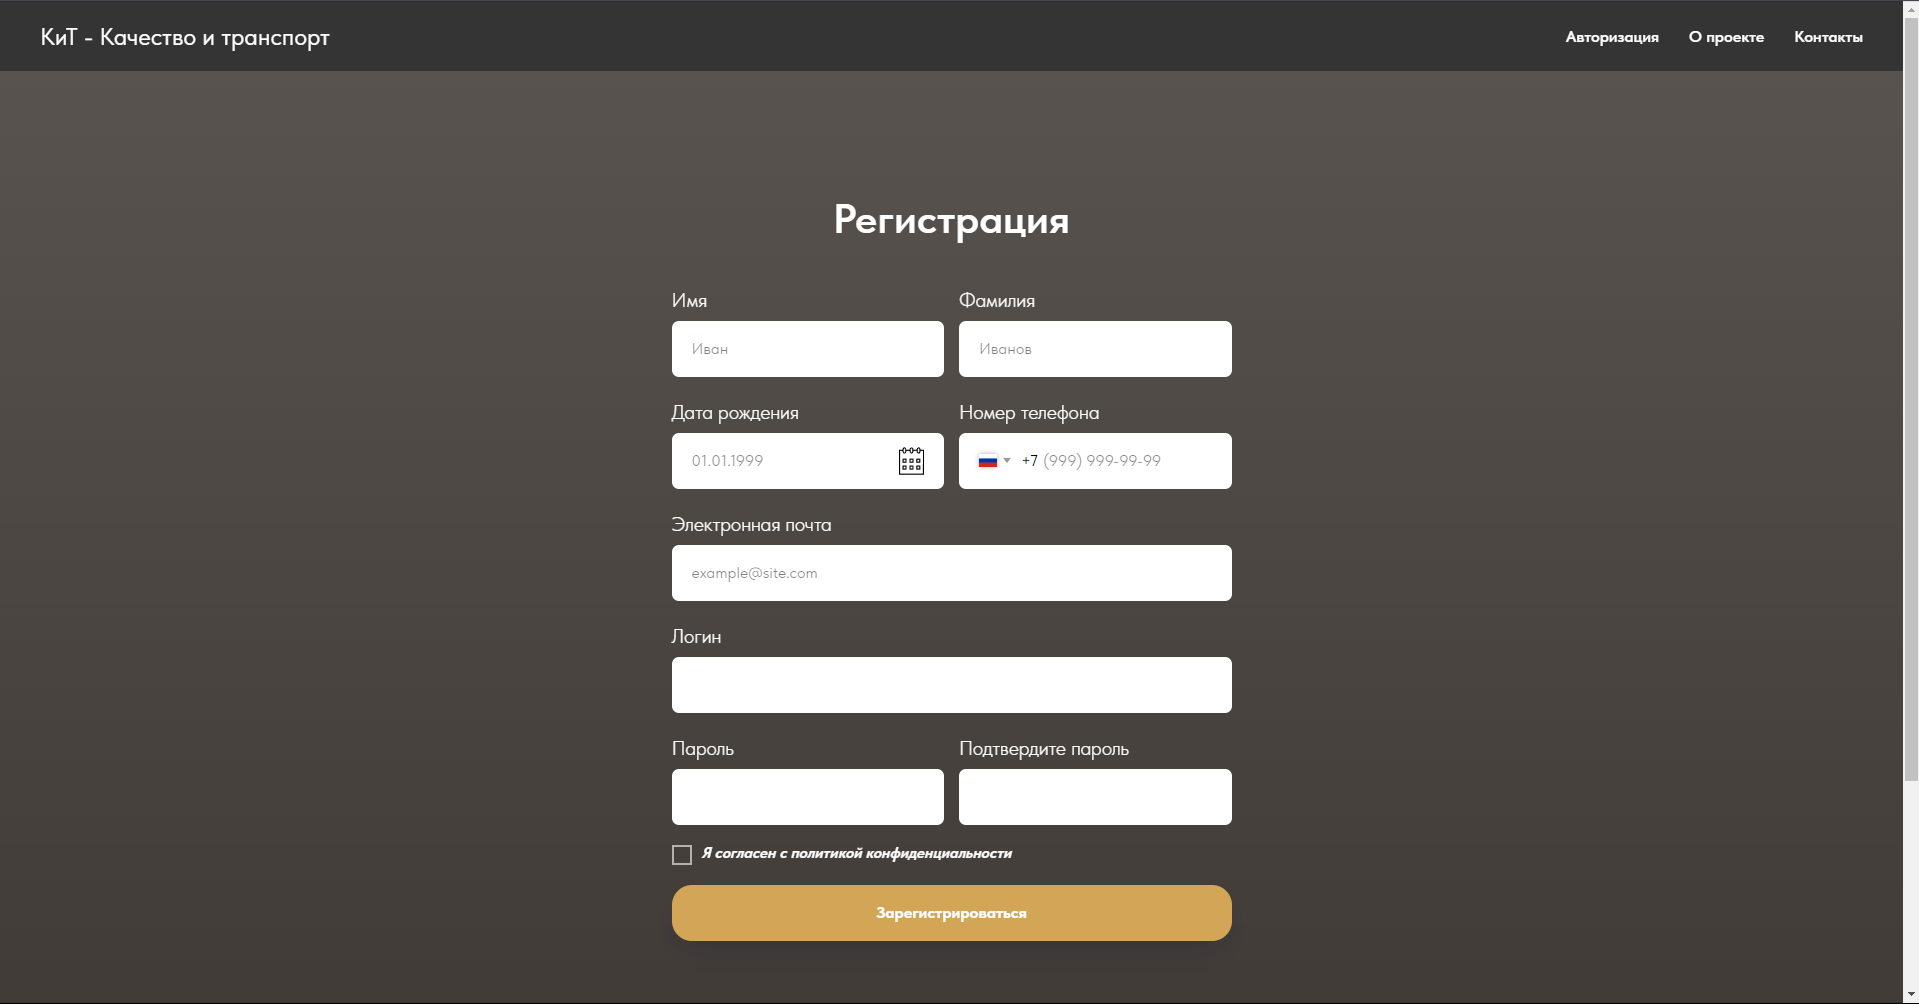
\includegraphics[width=1\linewidth]{Регистрация}
\caption{Макет формы регистрации}
\label{templ:image}
\end{figure}

\begin{figure}[H]
	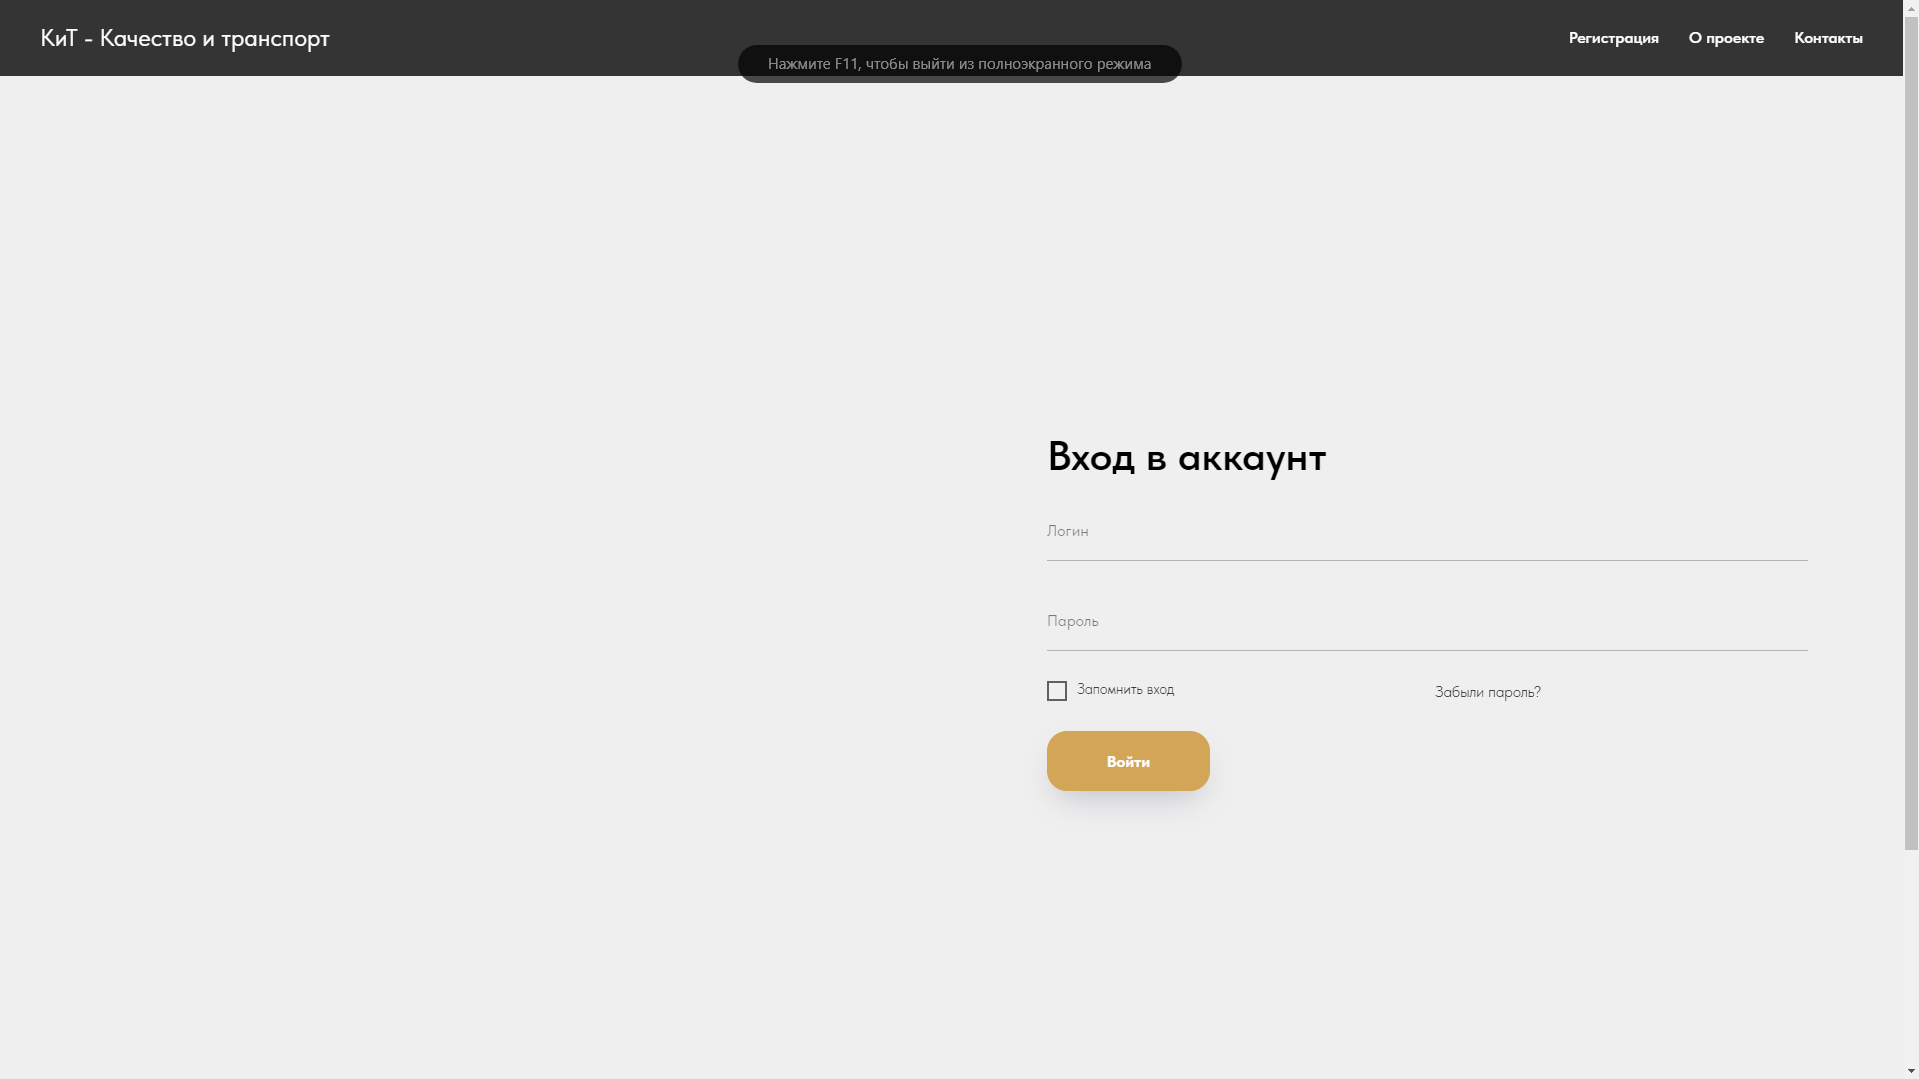
\includegraphics[width=1\linewidth]{Авторизация}
	\caption{Макет формы авторизации}
	\label{templ:image}
\end{figure}

\begin{figure}[H]
	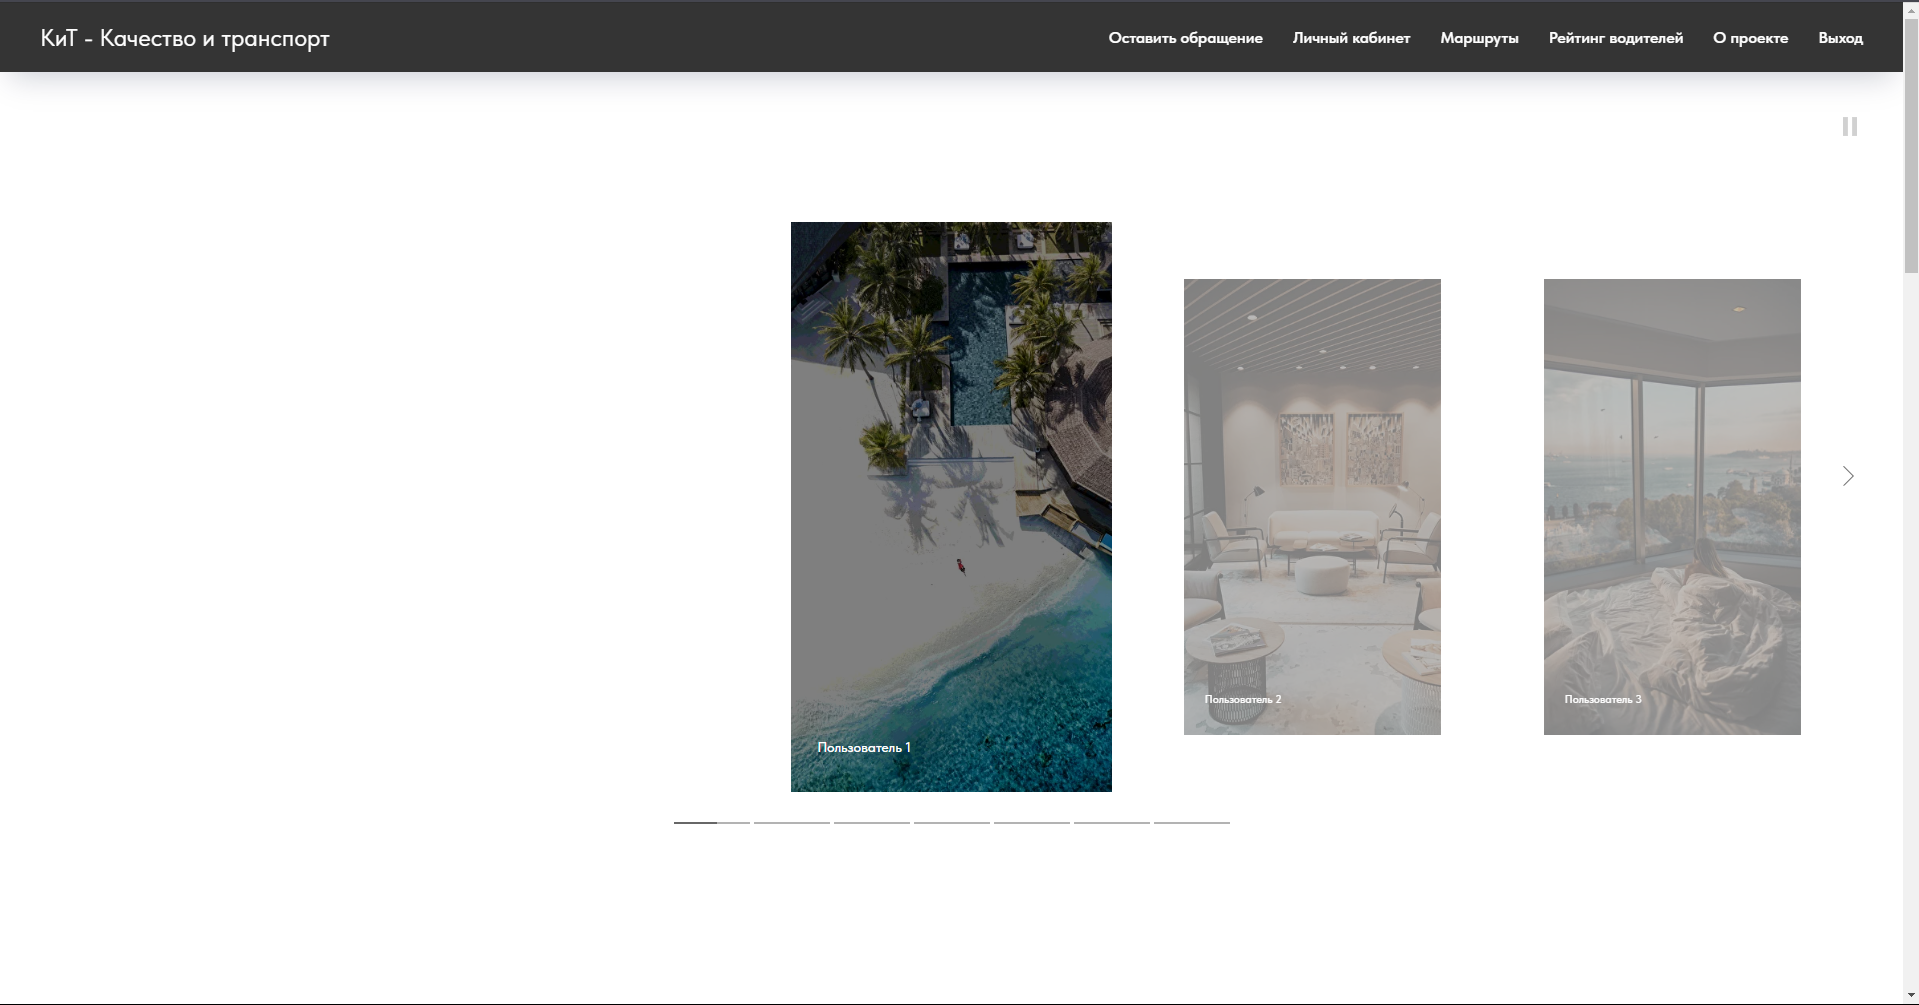
\includegraphics[width=1\linewidth]{Новостная лента}
	\caption{Раздел <<Новостная лента>>}
	\label{templ:image}
\end{figure}

\begin{figure}[H]
	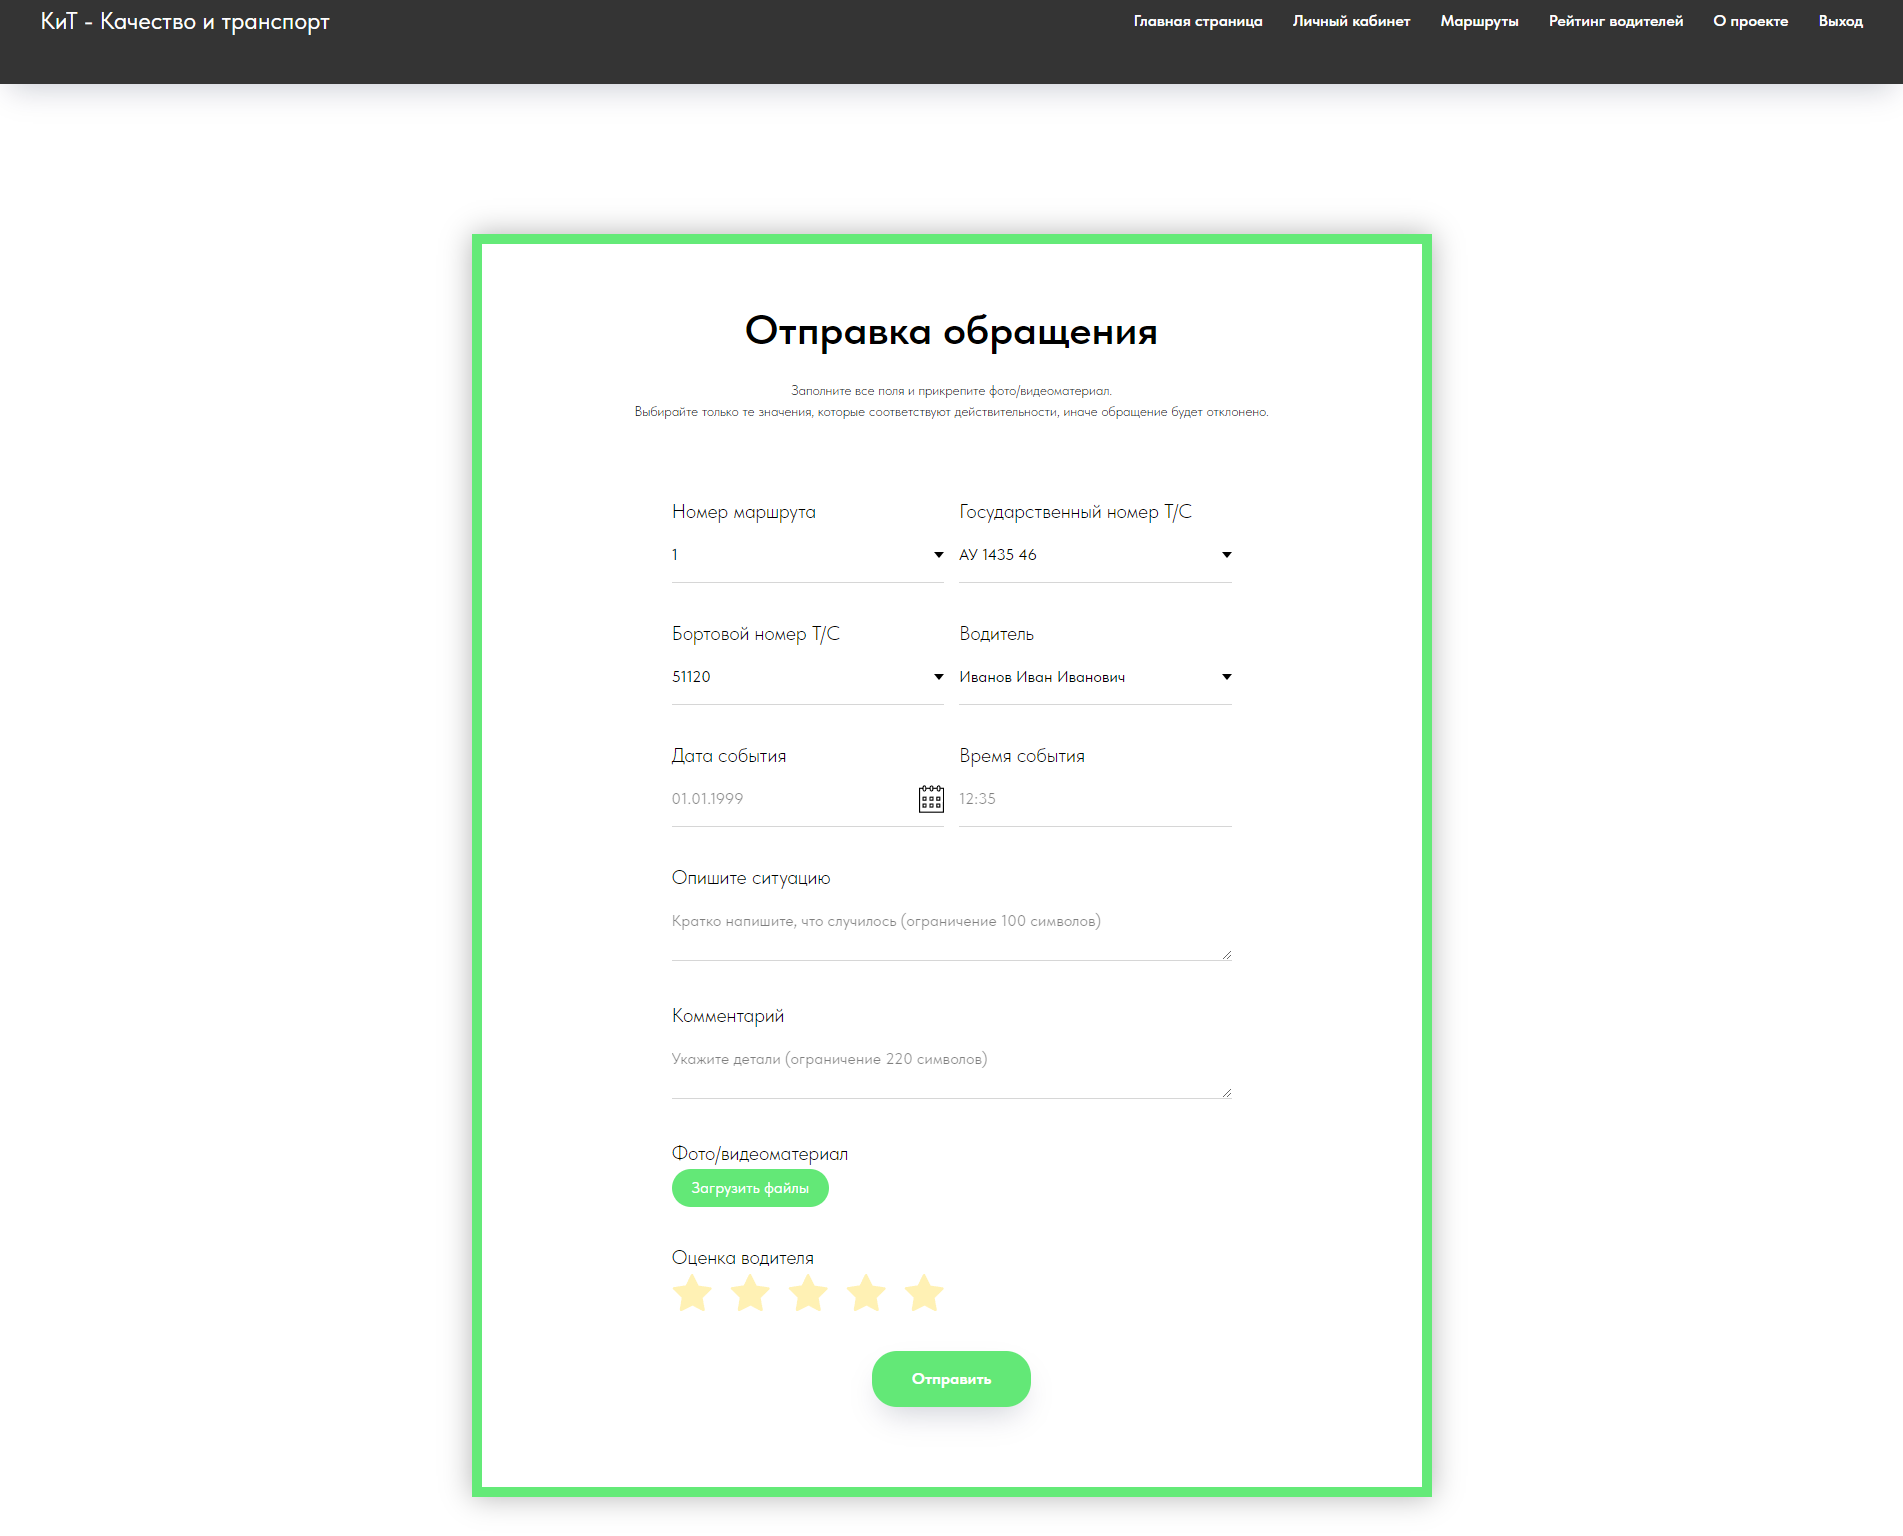
\includegraphics[width=1\linewidth]{Форма обращения}
	\caption{Раздел <<Отправка обращения>>}
	\label{templ:image}
\end{figure}

\subsection{Моделирование вариантов использования}

Для разрабатываемого веб-приложения была реализована диаграмма прецедентов - модель, обеспечивающая наглядное представление вариантов его использования. 

Она способствует физической разработке и детальному анализу взаимосвязей объектов. Для построения диаграммы вариантов использования применяется унифицированный язык визуального моделирования UML. 

Диаграмма вариантов использования описывает функциональное назначение разрабатываемой системы, то есть показывает, что система будет делать в процессе своего функционирования. Она представляет собой исходное концептуальное представление системы в процессе проектирования и разработки. В проектируемой системе прецеденты представляют собой действия, предоставляемые системой актерам или сущностям, взаимодействующим с системой. Актером является сущность, взаимодействующая с системой извне, будь то человек или техническое устройство. Прецедент описывает набор действий, которые система выполняет для актера.

На основании анализа предметной области в разрабатываемом веб-приложении сбора и анализа информации об инцидентах с общественным транспортом должны быть реализованы следующие прецеденты:
\begin{enumerate}
\item Регистрация аккаунта;
\item Авторизация пользователя;
\item Отправка обращений;
\item Публикация обращений;
\item Просмотр информации в личном кабинете;
\item Модерация обращений.
\end{enumerate}

На рисунке ~\ref{templ:image} представлены функциональные требования к системе в виде диаграммы прецедентов нотации UML.
\begin{figure}[H]
	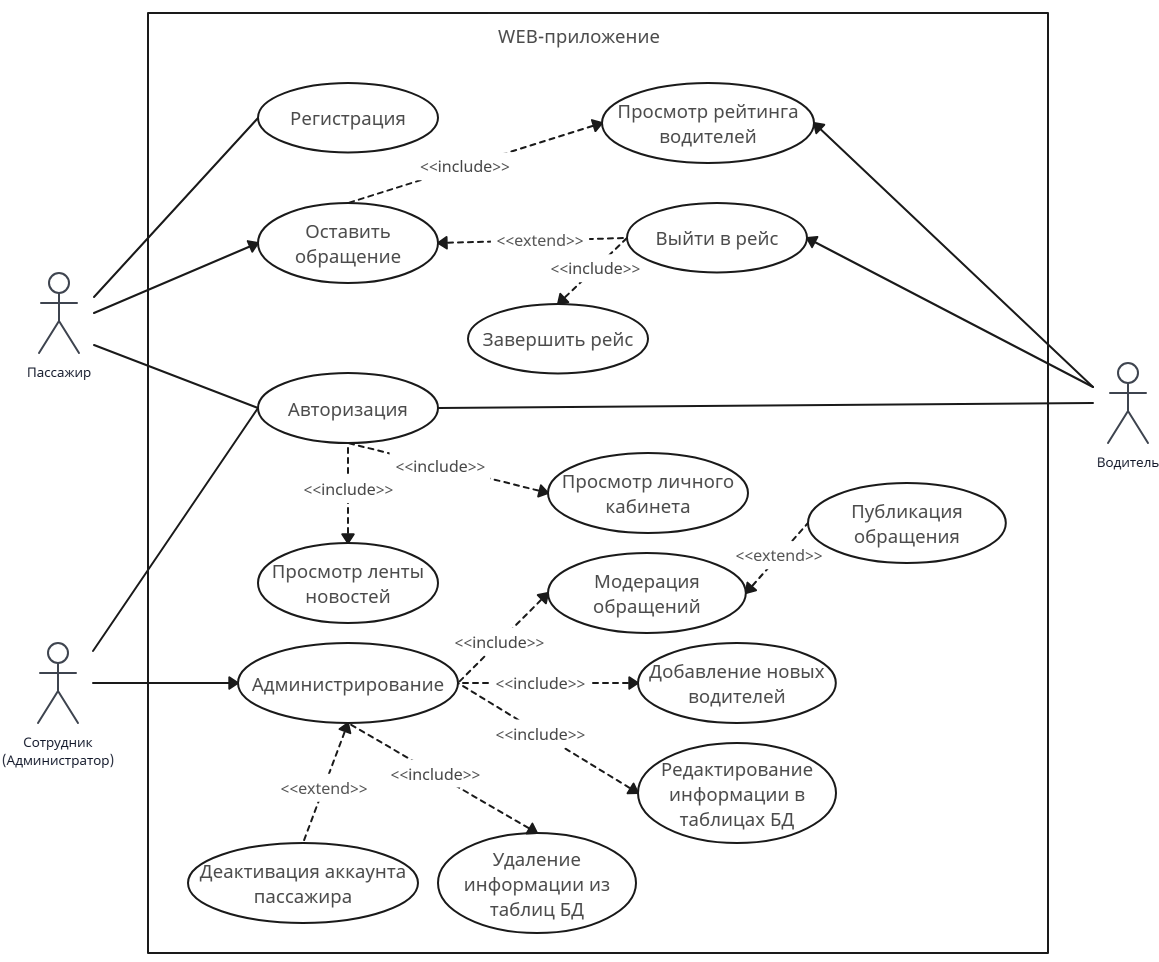
\includegraphics[width=1\linewidth]{Диаграмма прецедентов}
	\caption{Диаграмма прецедентов}
	\label{templ:image}
\end{figure}

\subsubsection {Вариант использования «Регистрация аккаунта»}
Заинтересованные лица и их требования: Пользователи, желающие получить доступ к веб-приложению.

Предусловие: Пользователь открывает страницу регистрации.

Постусловие: Пользователь имеет аккаунт в системе.

Основной успешный сценарий: 
\begin{enumerate}
\item Пользователь заходит на страницу регистрации.
\item Пользователь корректно заполняет все поля формы регистрации.
\item Пользователь нажимает на кнопку «Зарегистрироваться».
\item Система создает аккаунт пользователя.
\end{enumerate}

\subsubsection {Вариант использования «Авторизация пользователя»}
Заинтересованные лица и их требования: Пользователи, желающие получить доступ к веб-приложению.

Предусловие: Пользователь открывает страницу авторизации.

Постусловие: Пользователь попадает на главную страницу.

Основной успешный сценарий: 
\begin{enumerate}
	\item Пользователь заходит на страницу авторизации.
	\item Пользователь корректно вводит логин и пароль от своего аккаунта в соответствующих полях формы.
	\item Пользователь нажимает на кнопку «Войти».
	\item Система загружает главную страницу.
\end{enumerate}

\subsubsection {Вариант использования «Отправка обращений»}

Заинтересованные лица и их требования: Пользователи, желающие оставить обращение о случившемся инциденте.

Предусловие: Пользователь открывает раздел «Оставить обращение».

Постусловие: Пользователь отправляет обращение в систему.

Основной успешный сценарий: 

\begin{enumerate}
	\item Пользователь заходит в раздел «Оставить обращение».
	\item Пользователь заполняет все необходимые поля.
	\item Пользователь нажимает на кнопку «Отправить».
	\item Система создает новое обращение и отправляет его на проверку администратору.
\end{enumerate}

\subsubsection {Вариант использования «Модерация обращений»}

Заинтересованные лица и их требования: Пользователи, которые несут ответственность за корректность контента обращений.

Предусловие: Пользователь вошел в систему под своим аккаунтом, имеющим расширенные права доступа.

Постусловие: Пользователь допускает обращение для публикации.

Основной успешный сценарий: 

\begin{enumerate}
	\item Пользователь заходит в раздел «Новые обращения».
	\item Пользователь проверяет правильность введённых данных, а также содержание обращения на корректность и достоверность.
	\item Пользователь нажимает на кнопку «Опубликовать». 
	\item Система показывает обращение на главной странице с целью ознакомления для других пользователей.
\end{enumerate}

\subsubsection {Вариант использования «Просмотр информации в личном кабинете»}

Заинтересованные лица и их требования: Пользователи, желающие ознакомится или дополнить информацию о себе в личном кабинете.

Предусловие: Пользователь заходит в систему под своим аккаунтом. 

Постусловие: Пользователь просматривает или дополняет информацию о себе.

Основной успешный сценарий: 

\begin{enumerate}
	\item Пользователь заходит в раздел «Личный кабинет».
	\item Пользователь просматривает имеющуюся информацию и/или добавляет новую информацию.
	\item Пользователь нажимает на кнопку «Сохранить» при добавлении новых данных.
	\item Система выводит сообщение «Данные сохранены», при добавлении новых данных.
\end{enumerate}



\subsection{Требования к оформлению документации}

Разработка программной документации и программного изделия должна производиться согласно ГОСТ 19.102-77 и ГОСТ 34.601-90. Единая система программной документации.

\section{Технический проект}
\subsection{Общие сведения о программной системе}

Необходимо спроектировать и реализовать веб-приложение, которое будет предназначено для освещения инцидентов, связанных с общественным транспортом, таких как автобусы, троллейбусы и маршрутные такси. В веб-приложение предоставит пользователям возможность просматривать посты и видеозаписи, содержащие информацию об инцидентах с общественным транспортом. 

Для доступа к просмотру или оставлению обращений пользователи должны будут зарегистрироваться или войти в систему, что обеспечит контроль над контентом и позволит отслеживать активность каждого пользователя. Пользователи смогут оставлять свои обращения о случившихся инцидентах, заполняя форму обратной связи, где они будут описывать произошедшее событие. Зарегистрированные пользователи смогут просматривать все доступные посты и видеозаписи, связанные с инцидентами, которые будут отображаться в формате новостной ленты. Все оставленные обращения будут проходить обязательную модерацию, где тексты проверяются на отсутствие неподобающего контента. Только обращения, прошедшие модерацию, будут публиковаться в ленте.

Администраторы получат расширенные права доступа, позволяющие им добавлять новых водителей в базу данных, редактировать существующую информацию, а также управлять обращениями. Административная панель предоставит все необходимые инструменты для этих задач. В приложении будет предусмотрена функция отображения рейтинга водителей, что позволит пассажирам оценивать их работу и оставлять обратную связь. Пользователи также будут иметь доступ к личному кабинету, где они смогут управлять своей информацией, просматривать свои обращения и взаимодействовать с приложением. Это веб-приложение будет реализовано для освещения инцидентов, связанных с общественным городским транспортом, и будет служить платформой для обмена информацией между пассажирами и ответственными органами. 

Основная цель системы — предоставлять актуальные данные о происшествиях, чтобы ответственные службы могли оперативно реагировать на возникающие проблемы и улучшать качество обслуживания общественного транспорта.

\subsection{Проектирование архитектуры программной системы}

\subsubsection{Выбор архитектурного стиля и паттернов проектирования}

Архитектурный стиль и паттерны проектирования играют важную роль в создании высокопроизводительных, масштабируемых и безопасных систем, особенно когда речь идет о разработке REST API. REST API, или Representational State Transfer Application Programming Interface, представляет собой архитектурный стиль, который опирается на принципы унификации интерфейсов и передачи состояния между клиентом и сервером. При разработке REST API чрезвычайно важно правильно выбрать архитектурный стиль и использовать соответствующие паттерны проектирования, чтобы обеспечить эффективную работу системы и удовлетворить потребности пользователей.

Один из ключевых паттернов проектирования, который можно использовать при разработке REST API, - это паттерн Facade. Паттерн Facade позволяет создать унифицированный интерфейс для взаимодействия с комплексной системой, скрывая детали реализации и предоставляя простой и понятный интерфейс для внешних клиентов. Применение этого паттерна позволяет сделать REST API более модульным и гибким, упрощая его использование и поддержку.

Еще один важный паттерн - это Адаптер. В контексте REST API, Адаптер позволяет преобразовывать данные из одного формата в другой, обеспечивая совместимость между различными системами и источниками данных. Например, если данные получаются в формате, который необходимо преобразовать для работы с REST API, Адаптер может быть использован для выполнения этой задачи, обеспечивая единый формат данных для всей системы.

Клиент-серверная архитектура также играет важную роль в разработке REST API. Этот архитектурный стиль разделяет систему на две основные части: клиентскую сторону, которая отправляет запросы на сервер, и серверную сторону, которая обрабатывает эти запросы и возвращает результаты. Это позволяет создать масштабируемую и гибкую систему, которая может обрабатывать большие объемы запросов от множества клиентов одновременно.

Для обеспечения безопасности данных в REST API широко используются протокол HTTPS и технология ODBC (Open Database Connectivity). HTTPS обеспечивает защищенное соединение между клиентом и сервером, шифруя данные и предотвращая их несанкционированный доступ или изменение. ODBC, с другой стороны, предоставляет универсальный интерфейс для доступа к различным базам данных, позволяя безопасно и эффективно работать с данными в REST API.

Архитектура всей системы представлена на рисунке ~\ref{templ:image2}.
\begin{figure}[H]
	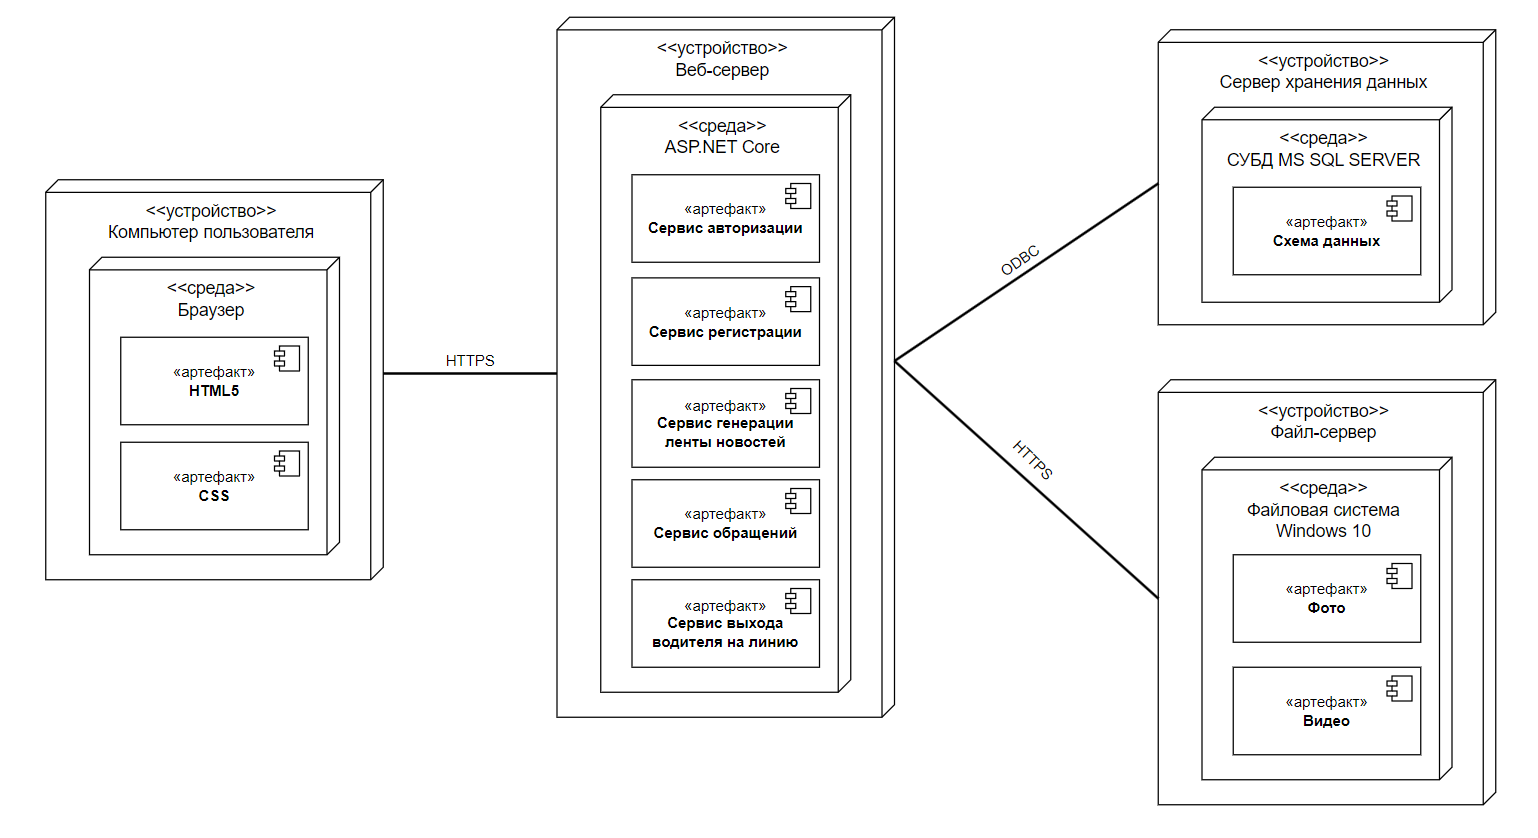
\includegraphics[width=1\linewidth]{Архитектура программной системы}
	\caption{Архитектура программной системы}
	\label{templ:image2}
\end{figure}

\subsubsection{Структура базы данных}

В качестве системы управления базами данных была выбрана реляционная СУБД Microsoft SQL Server. Она предназначена для хранения и управления данными, а также для выполнения различных задач по их обработке, анализу и управлению. SQL Server используется в корпоративных приложениях, веб-приложениях и других системах, где требуется надежное и масштабируемое хранилище данных.

Microsoft SQL Server обладает рядом преимуществ, которые делают его оптимальным выбором для управления базами данных в различных проектах. К ключевым преимуществам можно отнести:
\begin{itemize}
	\item Высокая производительность. SQL Server оптимизирован для высокой производительности как для транзакционных рабочих нагрузок, так и для аналитических запросов. Он включает в себя технологии, такие как in-memory processing и параллельное выполнение запросов, что позволяет обрабатывать большие объемы данных эффективно.
	\item Безопасность данных. SQL Server предоставляет обширные возможности для обеспечения безопасности данных. В него встроены функции шифрования данных, аутентификации, управления доступом на основе ролей (RBAC), а также средства для аудита и мониторинга безопасности.
	\item Высокая доступность и отказоустойчивость. Существует несколько функций для обеспечения высокой доступности и отказоустойчивости, включая Always On Availability Groups, репликацию и зеркалирование баз данных. Эти функции помогают минимизировать время простоя и обеспечивают непрерывный доступ к данным.
	\item Масштабируемость. SQL Server может масштабироваться как вертикально, так и горизонтально. Он поддерживает работу на разных уровнях — от небольших приложений до крупных корпоративных систем с большими объемами данных и высокой нагрузкой.
	\item Обширная поддержка и документация. Microsoft предоставляет обширную документацию, поддержку и ресурсы для обучения. Это включает в себя онлайн-документацию, форумы, обучающие курсы и официальные сертификации, что помогает администраторам и разработчикам быстро освоить и эффективно использовать SQL Server.
\end{itemize}

Несмотря на многочисленные преимущества, Microsoft SQL Server имеет и некоторые недостатки, которые могут быть значимыми в зависимости от конкретных требований и условий эксплуатации. К недостаткам можно отнести:
\begin{itemize}
	\item Обновления и совместимость. Обновления SQL Server могут вызывать затруднения и иногда могут создавать проблемы с совместимостью приложений, особенно если они зависят от определенных версий или функций базы данных. Это требует тщательного планирования и тестирования перед внедрением обновлений.
	\item Ограниченная кроссплатформенность. Хотя в последние годы Microsoft сделала шаги в сторону кроссплатформенности (например, выпустила версии SQL Server для Linux), основная платформа и многие функции SQL Server всё ещё оптимизированы для работы на Windows. 
	\item Требования к аппаратному обеспечению. Для достижения максимальной производительности SQL Server требует значительных ресурсов аппаратного обеспечения, таких как процессор, память и дисковое пространство.
\end{itemize}

На основании анализа предметной области и технического задания была разработана база данных, предназначенная для хранения и обработки хранящейся информации. Схема данных представлена на рисунке ~\ref{templ:image1}.
\begin{figure}[H]
	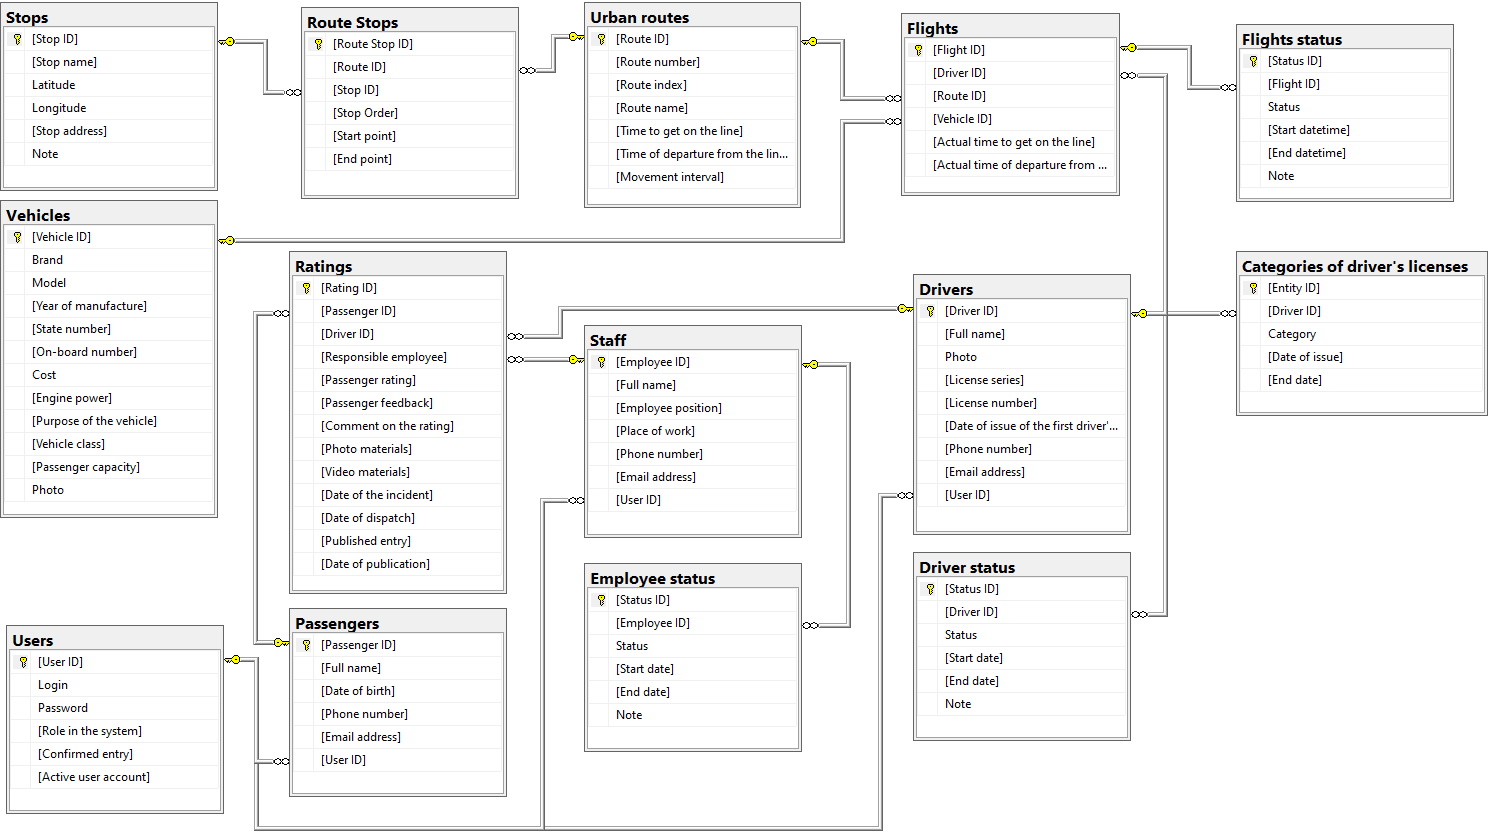
\includegraphics[width=1\linewidth]{Схема данных}
	\caption{Схема данных}
	\label{templ:image1}
\end{figure}

Все сущности базы данных приведены к третьей нормальной форме, что означает, что каждая таблица удовлетворяет требованиям нормализации:
\begin{enumerate}
	\item Отсутствие дублирования данных. В каждой таблице данные не дублируются, что помогает избежать избыточности и обеспечивает экономное использование ресурсов.
	\item Зависимость атрибутов от первичного ключа. Все неключевые атрибуты в таблице зависят только от первичного ключа, а не от других неключевых атрибутов. Это гарантирует, что каждая таблица содержит данные, относящиеся к одному логическому объекту или концепции.
	\item Устранение транзитивных зависимостей. Если атрибуты зависят друг от друга через другой атрибут, такие зависимости устранены. Это обеспечивает целостность данных и упрощает процесс обновления и удаления данных.
\end{enumerate}

Приведение базы данных к третьей нормальной форме помогает повысить эффективность запросов, уменьшить риск возникновения аномалий при обновлении данных и повысить отказоустойчивость.

\subsubsection{Описание микросервисов}
Микросервисы играют ключевую роль в разрабатываемом веб-приложении, поскольку они обеспечивают модульную архитектуру, гибкость и масштабируемость системы. Каждый микросервис представляет собой отдельную функциональную единицу, специализирующуюся на определенной задаче, что позволяет легко разрабатывать, развертывать и масштабировать приложение.
\begin{enumerate}
	\item Микросервис обработки обращений
	
	Назначение: Обработка обращений от граждан, связанных с инцидентами на общественном транспорте.
	
	Функции: Прием обращений, проверка корректности данных, направление обращений на модерацию администратору.
	
	Преимущества: Обеспечивает структурированное и оперативное управление обращениями, что способствует быстрому реагированию на проблемы и улучшению качества обслуживания пассажиров.
	
	\item Микросервис аутентификации и авторизации пользователей
	
	Назначение: Обеспечение безопасного доступа пользователей к веб-приложению.
	
	Функции: Управление регистрацией новых пользователей, проверка учетных данных при входе, назначение ролей и прав доступа.
	
	Преимущества: Гарантирует, что только авторизованные пользователи могут оставлять обращения и получать доступ к персонализированным функциям приложения, обеспечивая безопасность данных и предотвращение несанкционированного доступа.
	
	\item Микросервис работы с базой данных через панель администратора (управление базой данных)
	
	Назначение: Управление базой данных администратором системы.
	
	Функции: Добавление новых водителей в базу данных, редактирование и удаление информации, мониторинг активности пользователей, управление обращениями и отчетами.
	
	Преимущества: Обеспечивает администратору удобные инструменты для управления данными, что повышает эффективность администрирования и поддержания актуальности данных.
	
	\item Микросервис регистрации
	
	Назначение: Обеспечение удобного процесса регистрации новых пользователей в системе.
	
	Функции: Обработка регистрационных данных, проверка уникальности пользователей, отправка подтверждений по электронной почте.
	
	Преимущества: Облегчает процесс регистрации, повышая удобство для пользователей и увеличивая количество участников, активно использующих приложение.
\end{enumerate}

Эти микросервисы интегрированы для создания эффективной и надежной системы управления инцидентами в общественном транспорте. Они обеспечивают структурированный подход к обработке обращений, защиту данных, гибкость управления и удобство для конечных пользователей, что в конечном итоге способствует улучшению качества обслуживания и повышению доверия к транспортным службам.

\subsection{Обоснование выбора технологии проектирования}

В настоящее время информационный рынок, предоставляющий программные решения в выбранной сфере, предлагает множество продуктов, которые позволяют успешно разработать веб-приложение и достигнуть поставленной цели.

\subsubsection{Описание используемых технологий и языков программирования}

В процессе разработки веб-приложения используются различные программные средства и языки программирования, каждый из которых применяется для выполнения специфических задач, необходимых для реализации проекта.

\subsubsection{Язык программирования JavaScript}

Выбор языка программирования JavaScript для разработки микросервисов также обосновывается несколькими ключевыми преимуществами этого языка. Прежде всего, JavaScript является одним из самых популярных языков программирования, широко используемым в веб-разработке. Его широкое распространение обусловлено его универсальностью и возможностью использования как на стороне клиента (браузер), так и на стороне сервера (Node.js).

Второе важное преимущество JavaScript - его высокая гибкость и динамичность. JavaScript позволяет быстро создавать интерактивные и динамические пользовательские интерфейсы, что особенно важно для микросервисов, предоставляющих данные веб-приложениям.

Третье преимущество JavaScript - его асинхронная природа. JavaScript поддерживает асинхронное программирование, что позволяет эффективно обрабатывать большие объемы запросов и взаимодействовать с базами данных и другими внешними ресурсами без блокировки выполнения программы.

Наконец, JavaScript обладает обширной экосистемой библиотек и фреймворков, таких как Express.js для серверной разработки, React.js и Vue.js для разработки пользовательских интерфейсов, что делает его привлекательным выбором для создания микросервисных архитектур.

В целом, JavaScript представляет собой мощный инструмент для разработки микросервисов, обеспечивая высокую гибкость, производительность и возможность масштабирования системы.

\subsubsection{Язык программирования C\#}

Выбор языка программирования C\# для разработки микросервисов обусловлен несколькими ключевыми преимуществами этого языка. Прежде всего, C\# известен своей высокой производительностью, что обеспечивает быстрое выполнение программы. Второе важное преимущество - масштабируемость. С помощью C\# легко создавать системы, способные масштабироваться в соответствии с растущими потребностями. И наконец, кросс-платформенность делает C\# универсальным языком программирования, что позволяет разрабатывать приложения, работающие на различных операционных системах. Все эти факторы совместно обеспечивают быструю разработку надежной и масштабируемой системы при использовании C\#.

\subsubsection{HTML}

HTML является стандартным языком разметки, широко используемым для создания структуры веб-страниц. Выбор HTML для разработки микросервисов также имеет свои преимущества.

Во-первых, HTML является основным строительным блоком веб-страниц и обеспечивает их структуру и семантику. Это позволяет легко создавать пользовательские интерфейсы и представления для микросервисов, делая их интуитивно понятными и удобными для пользователей.

Во-вторых, HTML легко интегрируется с другими технологиями веб-разработки, такими как CSS для стилизации и JavaScript для создания интерактивных элементов. Это позволяет создавать более сложные и функциональные веб-приложения на основе микросервисной архитектуры.

Третье преимущество HTML - его доступность и поддержка во всех современных браузерах. Это обеспечивает широкий охват аудитории и упрощает развертывание и поддержку веб-приложений на основе микросервисов.

Наконец, HTML обладает простым и интуитивно понятным синтаксисом, что делает его доступным даже для новичков в веб-разработке. Это упрощает процесс создания и поддержки микросервисов, особенно при работе в команде.

В целом, HTML является важным инструментом для создания пользовательских интерфейсов и представлений в микросервисной архитектуре. Его простота, доступность и гибкость делают его привлекательным выбором для разработки веб-приложений любого уровня сложности.

\subsubsection{React}

React - это JavaScript-библиотека, разработанная для создания пользовательских интерфейсов веб-приложений. Выбор React для разработки микросервисов также имеет свои преимущества.

Во-первых, React предоставляет удобный и эффективный способ создания динамических пользовательских интерфейсов. Он использует компонентный подход, позволяя разбивать пользовательский интерфейс на множество небольших и переиспользуемых компонентов. Это делает код более чистым, модульным и легко поддерживаемым.

Во-вторых, React обеспечивает высокую производительность благодаря виртуальному DOM. Виртуальный DOM позволяет React оптимизировать обновление пользовательского интерфейса, перерисовывая только те компоненты, которые действительно изменились. Это делает React идеальным выбором для создания микросервисов с высокой производительностью и быстрой отрисовкой.

Третье преимущество React - его обширная экосистема. Существует множество дополнительных библиотек и инструментов, таких как Redux для управления состоянием, React Router для навигации в приложении, и многие другие, которые облегчают разработку микросервисов на основе React.

 React представляет собой мощный инструмент для разработки микросервисов, обеспечивая высокую производительность, модульность и широкие возможности для создания динамичных пользовательских интерфейсов.
\ifПрактика{}\else{
   \section{Рабочий проект}
\subsection{Классы, используемые при разработке сайта}

Можно выделить следующий список классов и их методов, использованных при разработке web-приложения (таблица \ref{class:table}). Пример таблицы с уменьшенным межстрочным интервалом.

\renewcommand{\arraystretch}{0.8} % уменьшение расстояний до сетки таблицы
\begin{xltabular}{\textwidth}{|X|p{2.5cm}|>{\setlength{\baselineskip}{0.7\baselineskip}}p{4.85cm}|>{\setlength{\baselineskip}{0.7\baselineskip}}p{4.85cm}|}
\caption{Описание классов Bitrix, используемых в приложении\label{class:table}}\\
\hline \centrow \setlength{\baselineskip}{0.7\baselineskip} Название класса & \centrow \setlength{\baselineskip}{0.7\baselineskip} Модуль, к которому относится класс & \centrow Описание класса & \centrow Методы \\
\hline \centrow 1 & \centrow 2 & \centrow 3 & \centrow 4\\ \hline
\endfirsthead
\caption*{Продолжение таблицы \ref{class:table}}\\
\hline \centrow 1 & \centrow 2 & \centrow 3 & \centrow 4\\ \hline
\finishhead
CMain & Главный модуль & CMain – главный класс страницы web-приложения. После одного из этапов по загрузке страницы в сценарии становится доступным инициализированный системой объект данного класса с именем \$APPLICATION & void ShowTitle(string property\_code = «title», bool strip\_tags = true)
Выводит заголовок страницы
void SetTitle(string title)
Устанавливает заголовок страницы

void ShowCSS(bool external = true, bool XhtmlStyle = true)
Выводит таблицу стилей CSS страницы\\
\hline CFile & Главный модуль & CFile – Класс для работы с файлами и изображениями & array GetFileArray (int file\_id)
Метод возвращает массив, содержащий описание файла (путь к файлу, имя файла, размер) с идентификатором file\_id
\end{xltabular}
\renewcommand{\arraystretch}{1.0} % восстановление сетки

\subsection{Модульное тестирование разработанного web-сайта}

Модульный тест для класса User из модели данных представлен на рисунке \ref{unitUser:image}.

\begin{figure}[ht]
\begin{lstlisting}[language=Python]
from django.test import TestCase
from .models import *
User = get_user_model()


class ShpoTestCases(TestCase):

    def setUp(self) -> None:
        self.user = User.objects.create(username='testtestovich', password='testtestovich', first_name='Sad', last_name='')

    def test_2(self):

        self.assertEqual(self.user.first_name, 'Sad')
        self.assertEqual(self.user.last_name, 'Cat')
        print((self.user))
        print((self.user.first_name))
        print((self.user.last_name))
\end{lstlisting}  
\caption{Модульный тест класса User}
\label{unitUser:image}
\end{figure}

\subsection{Системное тестирование разработанного web-сайта}

На рисунке \ref{main:image} представлена главная страница сайта «Русатом – Аддитивные технологии».
\newpage % при необходимости можно переносить рисунок на новую страницу
\begin{figure}[H] % H - рисунок обязательно здесь, или переносится, оставляя пустоту
\center{\includegraphics[width=1\linewidth]{main1}}
\center{\includegraphics[width=1\linewidth]{main2}}
\center{\includegraphics[width=1\linewidth]{main3}}
\caption{Главная страница сайта «Русатом – Аддитивные технологии»}
\label{main:image}
\end{figure}

На рисунке \ref{menu:image} представлен динамический вывод заголовков, включающий в себя искомые фразы при поиске фраз.

\begin{figure}[ht]
\center{\includegraphics[width=1\linewidth]{menu}}
\caption{Динамический вывод заголовков}
\label{menu:image}
\end{figure}

На рисунке \ref{enter:image} представлен ввод данных для публикации новости.

\begin{figure}[ht]
\center{\includegraphics[width=1\linewidth]{enter}}
\caption{Ввод данных для публикации очень-очень длинной, интересной и полезной новости}
\label{enter:image}
\end{figure}

   \section*{ЗАКЛЮЧЕНИЕ}
\addcontentsline{toc}{section}{ЗАКЛЮЧЕНИЕ}

Преимущества аддитивных технологий заключается в разнообразии процессов, позволяющих применять их в различных областях производства. Существенным ограничением же является и экономическая составляющая, которая не позволит внедрить аддитивное производство повсеместно.
  
Компании, видя, как развиваются информационные технологии, пытаются использовать их выгодно для своего бизнеса, запуская свой сайт для того, чтобы заявить о своем существовании, проинформировать потенциального клиента об услугах или продуктах, которые предоставляет. 
Для продвижения компании «Русатом – Аддитивные технологии» был разработан веб-сайт на основе системы «1С-Битрикс: Управление сайтом».

Основные результаты работы:

\begin{enumerate}
\item Проведен анализ предметной области. Выявлена необходимость использовать 1С-Битрикс.
\item Разработана концептуальная модель web-сайта. Разработана модель данных системы. Определены требования к системе.
\item Осуществлено проектирование web-сайта. Разработана архитектура серверной части. Разработан пользовательский интерфейс web-сайта.
\item Реализован и протестирован web-сайт. Проведено модульное и системное тестирование.
\end{enumerate}

Все требования, объявленные в техническом задании, были полностью реализованы, все задачи, поставленные в начале разработки проекта, были также решены.

Готовый рабочий проект представлен адаптивной версткой сайта. Сайт находится в публичном доступе, поскольку опубликован в сети Интернет.  

}\fi
\addcontentsline{toc}{section}{СПИСОК ИСПОЛЬЗОВАННЫХ ИСТОЧНИКОВ}

\begin{thebibliography}{9}

    \bibitem{javascript} Фримен, А. Практикум по программированию на JavaScript / А. Фримен. – Москва~: Вильямс, 2013. – 960 с. – ISBN 978-5-8459-1799-7. – Текст~: непосредственный.
    \bibitem{php} Бретт, М. PHP и MySQL. Исчерпывающее руководство / М. Бретт. – Санкт-Петербург : Питер, 2016. – 544 с. – ISBN 978-5-496-01049-8. – Текст~: непосредственный.
    \bibitem{css} Веру, Л. Секреты CSS. Идеальные решения ежедневных задач / Л. Веру. – Санкт-Петербург : Питер, 2016. – 336 с. – ISBN 978-5-496-02082-4. – Текст~: непосредственный.
    \bibitem{mysql}	Гизберт, Д. PHP и MySQL / Д. Гизберт. – Москва~: НТ Пресс, 2013. – 320 с. – ISBN 978-5-477-01174-2. – Текст~: непосредственный.
	\bibitem{html5}	Голдстайн, А. HTML5 и CSS3 для всех / А. Голдстайн, Л. Лазарис, Э. Уэйл. – Москва~: Вильямс, 2012. – 368 с. – ISBN 978-5-699-57580-0. – Текст~: непосредственный.
	\bibitem{htmlcss}	Дэкетт, Д. HTML и CSS. Разработка и создание веб-сайтов / Д. Дэкетт. – Москва~: Эксмо, 2014. – 480 с. – ISBN 978-5-699-64193-2. – Текст~: непосредственный.
	\bibitem{bigbook}	Макфарланд, Д. Большая книга CSS / Д. Макфарланд. – Санкт-Петербург : Питер, 2012. – 560 с. – ISBN 978-5-496-02080-0. – Текст~: непосредственный.
	\bibitem{uchiru}	Лоусон, Б. Изучаем HTML5. Библиотека специалиста / Б. Лоусон, Р. Шарп. – Санкт-Петербург : Питер, 2013 – 286 с. – ISBN 978-5-459-01156-2. – Текст~: непосредственный.
	\bibitem{chaynik}	Титтел, Э. HTML5 и CSS3 для чайников / Э. Титтел, К. Минник. – Москва~: Вильямс, 2016 – 400 с. – ISBN 978-1-118-65720-1. – Текст~: непосредственный.    
	\bibitem{22}	Титтел, Э. HTML5 и CSS3 для чайников / Э. Титтел, К. Минник. – Москва~: Вильямс, 2016 – 400 с. – ISBN 978-1-118-65720-1. – Текст~: непосредственный.    
	\bibitem{1231}	Титтел, Э. HTML5 и CSS3 для чайников / Э. Титтел, К. Минник. – Москва~: Вильямс, 2016 – 400 с. – ISBN 978-1-118-65720-1. – Текст~: непосредственный.    
	\bibitem{sdf}	Титтел, Э. HTML5 и CSS3 для чайников / Э. Титтел, К. Минник. – Москва~: Вильямс, 2016 – 400 с. – ISBN 978-1-118-65720-1. – Текст~: непосредственный.    
	\bibitem{servsssds}	Титтел, Э. HTML5 и CSS3 для чайников / Э. Титтел, К. Минник. – Москва~: Вильямс, 2016 – 400 с. – ISBN 978-1-118-65720-1. – Текст~: непосредственный.
\end{thebibliography}

\ifВКР{\appendix{Представление графического материала}

Графический материал, выполненный на отдельных листах,
изображен на рисунках А.1--А.\arabic{числоПлакатов}.
\setcounter{числоПлакатов}{0}

\renewcommand{\thefigure}{А.\arabic{figure}} % шаблон номера для плакатов

\begin{landscape}

\begin{плакат}
    
\includegraphics[width=0.82\linewidth]{плакат1.png}
    \заголовок{Сведения о ВКРБ}
    \label{pl1:image}      
\end{плакат}

\begin{плакат}
    
\includegraphics[width=0.82\linewidth]{плакат2.png}
    \заголовок{Цель и задачи разработки}
    \label{pl2:image}      
\end{плакат}

\begin{плакат}
    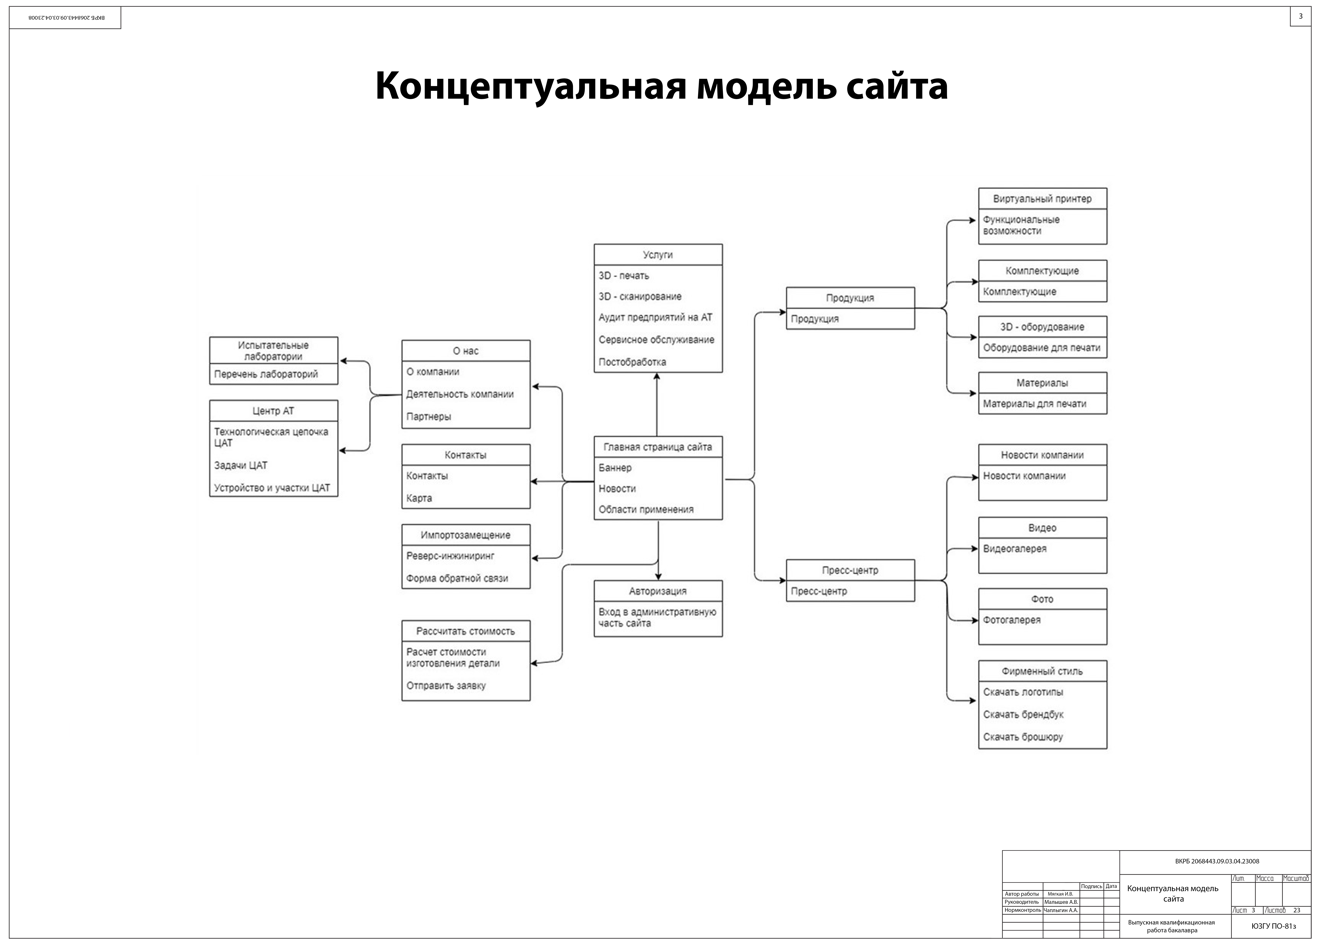
\includegraphics[width=0.82\linewidth]{плакат3.png}
    \заголовок{Концептуальная модель сайта}
    \label{pl3:image}      
\end{плакат}

\begin{плакат}
    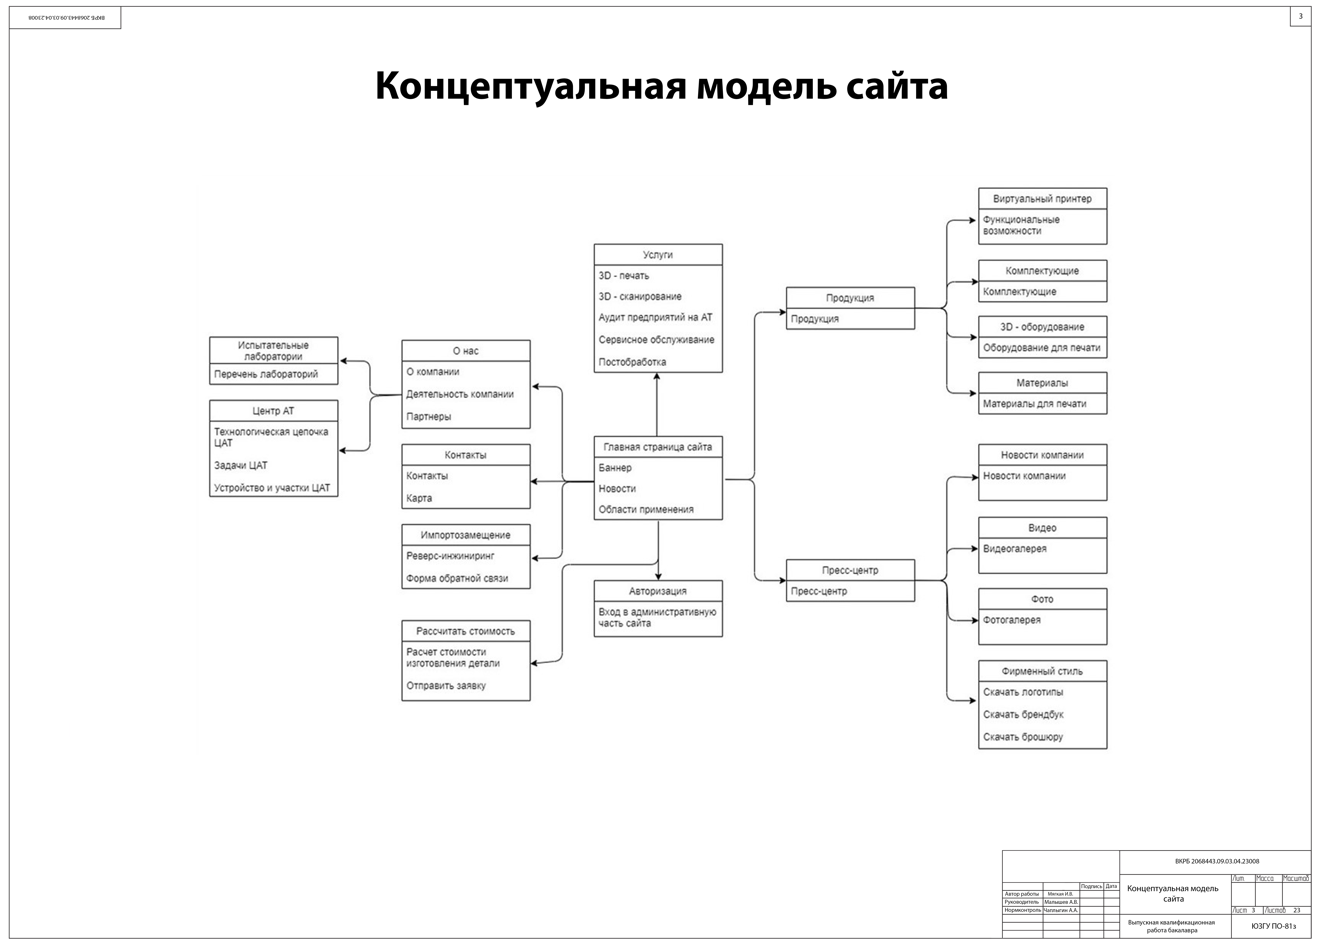
\includegraphics[width=0.82\linewidth]{плакат3.png}
    \заголовок{Еще плакат}
    \label{pl4:image}      
\end{плакат}

\end{landscape}
}\fi
\ifПрактика{}\else{\appendix{Фрагменты исходного кода программы}

main.tex
\lstinputlisting[language=Tex, frame=none]{main.tex}

ТехПроект.tex
\lstinputlisting[language=Tex, frame=none]{ТехПроект.tex}

\ifВКР{
\newpage
\addcontentsline{toc}{section}{На отдельных листах (CD-RW в прикрепленном конверте)}
\begin{center}
\textbf{Место для диска}
\end{center}
}\fi
}\fi
\end{document}
